%\documentclass[man]{apa}
%\documentclass[doc]{article}{styles/apacls/apa}
%\documentclass{report}
%\documentclass[man]{styles/apacls/apa}

%\documentclass[11pt,twoside,a4paper]{article}
%\documentclass[11pt,twoside,a4paper]{book}
%\documentclass[11pt,twoside,a4paper,openright]{report}
\documentclass[11pt,oneside,a4paper,openright]{report}

\usepackage{mathptmx}       % selects Times Roman as basic font
\usepackage{helvet}         % selects Helvetica as sans-serif font
\usepackage{courier}        % selects Courier as typewriter font
\usepackage{type1cm}        % activate if the above 3 fonts are
                            % not available on your system
\usepackage[utf8]{inputenc}
\usepackage{textcomp}
\usepackage{makeidx}         % allows index generation
\usepackage{graphicx}        % standard LaTeX graphics tool
                             % when including figure files
\usepackage{multicol}        % used for the two-column index
\usepackage[bottom]{footmisc}% places footnotes at page bottom

\usepackage{verbatim}        % per comentaris multilinia
\usepackage[utf8]{inputenc} %permite escribir {\'a},{\'e},{\'u},{\'o},{\'\i} & {\~n} directamente
\usepackage[british]{babel}
\usepackage{csquotes}
\usepackage{amsmath, amsthm, amssymb}
\usepackage{enumerate}
\usepackage{algorithm2e}
\usepackage{pdfcomment}
%\usepackage[lined,boxed,commentsnumbered]{algorithm2e}


\begin{document}
\title{Coevolutionary strategies in MultiAgent systems. An approach using socionatural realistic environments.\\
\small{Master Thesis}}
\author{Alexis Torrano Mart\'inez}
\maketitle
\newpage

%\textwidth 6in \oddsidemargin 0.2in \evensidemargin -0.2in
%\textheight 9in \topmargin -0.75in \headheight 0mm \headsep 25mm

%\Large
%\addtolength{\hoffset}{-2cm}

\pagenumbering{roman}
\begin{abstract}
The aim of this master thesis is the development of a multiagent model for a simulation of two populations whose interactions are strongly influenced by a realistic landscape.
This research will be in line with Consolider-Simulpast (www.simulpast.es), an interdisciplinary project aimed to create simulations designed to be used in archaeological studies of human-environment interaction, decision-making processes and coevolutionary/competition behaviours of past societies.
The work plan will be focused on the development of first-stage models for two societies in the age of agriculture spreading surpasing the hunting and foraging way of living. The simulation will involve a climate engine for seasonality depending primarily on variable rainfall rate. Landscape information will be created from satellite image rasters. Constants, and variable relationship shall be modelled from measures and interviews with the experts. Data analysis tasks will be undertaken to validate the models and detect patterns in the archaeological record. Furthermore a comparison will be stablished between the classical simple models used in social simulation[1][2][8] and more advanced approaches.
\end{abstract}
\newpage 

\setcounter{tocdepth}{6}
\tableofcontents
\newpage 

\pagenumbering{arabic}
\chapter{Introduction}

\section{Description}

%Problem, Gujarat, Archeology (com al resum de la matri­cula).

\section{Motivation}

Simulation has been following an evolution in the models and paradigms applied to represent its target
systems. Dynamical systems, differential equations have been used and an overall simplification of the parts of the systems in the history of simulation to operate with the abstraction and simplification of the problems.
Mainly, reusing ideas from physical simulations, social sciences has modelled complex systems with dynamical
atomic entities that apply a simple set of centralized rules to move around the environment modelled. It was seen that due to the deeper details in human behaviour the question that could be solved and asked to that kind of models could not go very further as expected.\\ 

To solve non-linearity phenomena, heterogeneity, hysteressis and other issues typical of complex systems, Agent Based Models(ABMs) where introduced to gain more insight of the modelled systems achieving good results. But under 
some conditions of very complex relationships between agents, highly specialized decission taking procedures
and issues in the environment led agents to need a sophysticated reasoning and problem solving capabilities
that are not specified and not yet introduced in ABMs coming from Social Sciences.\\ 

We have found an example of that situation in our case study located in Gujarat from Simulpast project. Our agents must interact with a regular but changing environment to get resources, plan its actions, coordinate with its group and compete with other groups in a \textbf{co-evolution} dynamic. Because we want to find out why the Gujarat HunterGatherer(HG) way of life lasted more than in other place of Earth in its competition against AgroPastoralist(AP), we need to embed the behaviours of the survival strategies used by these groups. A simply reactive agent cannot cope with short term plus long term decissions in that competitive environment. So the question stated as topic for this Master Thesis project is \textbf{``do we get better results in social sciences simulations adding deeper AI techniques to make richer the behaviour or decission making engines of the entities in the system?''}. As we understand ``better results``, the outcome from the use of AI should be a more sound validation of the model, a nearier match of modelled behaviours with the real ones, and clearer, richer and robust scientific conclusions.\\

In order to study such posibilities Sugarscape is a good framework to extend. Sugarscape is an artificial society developed by Joshua Epstein et al \cite{EpsteinAxtell}. where a number of inhabitants move to collect resources they need to live. Sugarscape models perception, lattice scanning in search of resources, sexual reproduction of the agents in the simulation, market relationships, immunology and spreading of diseases, and feature evolution. Epstein analises different experiments executed in the Sugarscape offering his conclusions and the dynamics emerging from the simulations. The results and conclusions will feed our AI experiments in order to make the comparisons of classical SugarScape agents vs AI agents, therefore, giving an answer to the topic of the Master Project.\\

\section{Simulation}

%brief description
%hi ha altres aplicacions de simulacio on no hi ha component temporal i no ho estic esmentant! MonteCarlo,etc...
Simulation is a discipline for performing virtual experiments in a computer. Computational techniques are used to build a model that represents your system. The dynamics of that system is codified in an algorithm that computes a calculus imitating the changes of state in the model, hence having a representation of that change along the time of the system modelled. Simulate is to play to ''what happens if...?'', and it is aimed to discover and explain the dynamics of a system to enhace or guide strategy development, decission taking, management, solving problems without analytical solutions or knowledge discovering and research. Although, we could get other positive benefits from it like theory checking or training through the inmersion in virtual worlds responding to our input.\\
% purpose, a priori, outcome, { deduction, induction, abduction(Alexis) } Axelrod's
% crec que els agradara, marketing, saborcillo de IA impregnant els racons
A simulation obeys some direction of experimentation, so a question must be set to drive the selection of features to model from the real system and give a direction to the modelling and the experiments design.These assumptions choice will prune the details not related to the questions to solve. It is not just for the sake of simplicity but for the practical reason that a model too near of the real system will be as hard as the original system to analyse.\\
Simulation, like deduction, starts with a set of those explicit assumptions. But unlike deduction, it does not prove theorems. Instead, a simulation generates data that can be analysed inductively. Unlike typical induction, however, the simulated data comes from a rigorously specified artificial experiment rather than direct measurement of the real world. While induction can be used to find patterns in data, and deduction can be used to find consequences of assumptions, simulation modelling can be used as an aid intuition and hypothesis validation tool. Also as space search mechanism for parameter tunning or optimization. This links with abductive processes.\\
%abduction
Just like in a tipical Sherlock Holmes case you pick the evidences, scenario for the experiment, and the common knowledge (the initial expert assumptions about the model). You enter in a refinement cycle where you test hypothesis and readjust them to discover the theory, the ``plot'', the explanation of what is happening. Following the abductive reasoning schema one looks for the hypothesis that would best explain the relevant evidence \cite{Axelrod2003}.\\
%% no anava errat amb l'abduccio! :D

%--: simulation, results, validation and statement of your inital hypothesis and question...
%--: simulation connected to abduction
% connect abduction with the simulation lifecycle 

Social simulation is a research field that applies computational methods to study issues in the social sciences. The issues explored include problems in psychology, sociology, political science, economics, anthropology, geography, archaeology and linguistics \cite{TakahashiSallachRouchier2007}.\\
Social simulation aims to cross the gap between the descriptive approach used in the social sciences and the formal approach used in the hard sciences, by moving the focus on the processes/mechanisms/behaviors that build the social reality.\\
In social simulation, computers supports human reasoning activities by executing these mechanisms. This field explores the simulation of societies as complex non-linear systems, which are difficult to study with classical mathematical equation-based models.
%reducibility 
Most of the times, studying complex systems implies to cope with non reducibility. One of the examples is Gravitational Dynamics. If our assumption is the use of Newton's mechanics, we can predict the state at any time or not, depending on the scenario. For a one dimension world you can predict the state at time $t_n$ from the initial state $t_0$ without computing all the preceding ones. For two and more dimensions you can only compute directly state $t_n$ if less the three bodies are implied. So in a real environment of many bodies in a 3D world you need to compute all the states from the initial to the one you consider as the last one. The system is non analytically reducible and you are forced to apply simulation to visit all the states and develop the behaviour of the model. It happens in most of the complex systems models, they have a nonlinear specification. Nonlinear models do not have a simple or computational reasonable analytical solution. 
% ( Classical Physics formulae used are non linear, acceleration is a quadratic factor in position <-- revisa aquesta fantasmada ) 

%emergence
Other of the main issues in complex systems simulation is emergence. While the initial assumptions may be simple, the consequences may not be at all obvious. The large-scale effects of locally interacting entities are called "emergent properties" of the system. Emergent properties are often surprising because it can be hard to anticipate the full consequences of even simple forms of interaction. 

%why simulation? because I need this non deducible emergence and the non deducible end state
There are some models, however, in which emergent properties can be formally deduced. Good examples include the neo-classical economic models in which rational agents operating under powerful assumptions about the availability of information and the capability to optimize can achieve an efficient reallocation of resources among themselves through costless trading. But when the agents use \textbf{adaptive} rather than optimizing strategies, deducing the consequences is often impossible; simulation becomes necessary.
% i ara estic preparat per conectar amb Social Science Simulation : reducibility + emergence forces to use simulation in S.S.

% Applying Simulation in the framework of Social Sciences to approach to the hypothesis of Simulpast targets, in concrete, about the case study from Gujarat, CS1.
%
%simulacio de sistemes complexes : f\'isica de particules, mercats, ... ecologia i... social sciences...
%
%n-body problem
%  2 body : formula
%  n body in 2D  : formula
%  n>2 body in 3D : simulation, non reducible
%   gravitation, electrostatics : input=initial position, output=end position, classical physics formulae: non linear!!!
%   acceleration is a quadratic factor in position!!!
%
%mes endevant cal caracteritzar la simulació : deterministic/stochastic, static/dynamic, open/closed, %linear/nonlinear, hysteressis, stable/unstable,
%stationary stage, emulation/monteCarlo/traceDriven/DiscreteEvent/DiscreteUnitTimeStep
%
%
%
%
\section{Question} 

% trobo a faltar m\'es xixa te\`orica, aix\`o s'hauria de semblar m\'es a un cap\'itol del Norvig.
In classical simulation approaches, specifically in the branch of Social Simulation, active entities which model human actors are designed with very simple behaviour engines. The classical hypothesis is that a complex mind for entities in the simulation are not that needed and maybe even could lead to difficult analysis of final results of the simulations (too daring statement?). 

Our statement is that, on the contrary, the mind engine of a simulation entity should not be bounded to that limit but special attention must be paid to give any necessary sofistication to give the entity a correct behaviour, real enough, sensible to the changes in the environment and competent to solve the issues that will have to solve along its lifetime in the system. Even more, we think that this entities' capability to respond with complex behaviours is the core that roots the modelling granularity needed to catch the essential of the social systems that we want to model.
%TODO ( a l'apartat de ABMs ho tornem a dir però afegint que cal adaptabilitat, resposta no lineal, aprenentatge depenent del temps, histeresis,...).\\
%( i aixo motivaria els ABMs) 
Applying such premises we will explore the possibility to give or enhance decission making, problem solving
capabilities to the entities with the aim to get more accurate simulations and realistic models with higher matching against our job hypothesis and premises. We will take the framework of ABMs to integrate the AI techniques in a decission making schema of action-response dynamics sensible to a modelled world.\\

%% ABM -> Decentralization of Decision-Making

%%exposicio mes detallada dels punts febles que creus que trobaràs als simple agents (i a les conclusions 
%% d'AI-Sugarscape se't confirma 
%% i d'altres outcomes)

\indent \textbf{Do AI techniques contribute to better simulation results?}\\
\indent \textbf{Classic Simple Agent approach vs Rich Agents}\\
\indent \textbf{Did Gujarat extreme enviromental conditions delayed the HG disappearence?}\\
\newpage 




\chapter{Methodology}

% on poso els steps del modelling procedure????
% specificacion --> expert's knowledge --> modelling --> prototipe --> { accept model | go to a previous state }
% revisiting early stages to refine models : toy model --> reviewing your assumptions about the main purpose
% interviews and ecotono meetings to motivate and help knowledge extraction
% ecotono modellings as a means to gain insight of the problem and the system, inspirational ideas.


\section{Intro}

%% metode = modelling\\
%% tecnica en ciencies socials = ABMs \\
%% afegir capitol llibre Rub+Cris\\

%que es modelling en ciencies socials 

% ATM mini intro

%hi ha un problema, analitzar-lo per solventar-ho, rational activity -> models

Modelling is a widely extended methodology to answer the kind of questions we set out. It comes from the natural observation of the world and the curiosity or need to reproduce it.\\
The modelling activity determines aspects of the world to include or exclude from the details that
will conform an abstraction of the world that will allow work the answers \cite{Robinson2008}.
%TODO multiple ref resuse : split in chapters/paragraphs

%% Robinson2008
%% In broad terms, conceptual modelling is the process of ab-
%% stracting a model from the real world. The modeller is pre-
%% sented with a problem situation that is amenable to simula-
%% tion modelling and then has to determine what aspects of
%% the real world to include, and exclude, from the model, and
%% at what level of detail to model each aspect. These deci-
%% sions should generally be a joint agreement between the
%% modeller and the problem owners i.e. the stakeholders who
%% require the model to aid decision-making.

%% >>> conceptual modelling is the process of ab-
%% stracting a model from the real world.

%% >>>then has to determine what aspects of
%% the real world to include, and exclude, from the model, and
%% at what level of detail to model each aspect.

%% \cite{Robinson2008}

%%Pidd
%% Models are convenient worlds. They are artificial worlds that have been deliberately 
%% created to help with understanding the possible consequences of particular actions. 
%% They are part of a process of ‘‘reflection before action’’ (Boothroyd, 1978). The 
%% models may be quantitative or qualitative, but in any case they will be simplified 
%% abstractions of the system of interest.

%% >>>> They are artificial worlds that have been deliberately 
%% created to help with understanding the possible consequences of particular actions.

%% >>>> The models may be quantitative or qualitative, but in any case they will be simplified 
%% abstractions of the system of interest.

%% \cite{Pidd2003}

Modelling will be our framework for communication between archeologists' and sociologists' knowledge and their conceptualizations with our formal representations from computer science practices( simulation, algorithms, AI ).
The reason is that it is a procedure that will help to communicate the \textbf{discursive} nature of Social Sciences with the formal structures from Computer Science. The enginering of model development will allow us to reach a connection from experts' knowledge to a model that comprises the set of detail clearing out the ambiguity that language could filtrate. Also, modelling will help set a picture of the system without inconsistencies, with each fact sound, coherent and consistent from the logical point of view with the whole.\\ 

\section{Why model}
% ATM, que es modelar? i com es modela?
%
The modelling process consists in identifying separable entities, processes, relationships and any rellevant information related to the question to solve and the domain of study. 
This abstraction exercise yields an external and explicit representation of part of reality as seen by the
people who wish to understand, to change, to manage or to control that part of reality \cite{Pidd2003}.\\
Indeed just thinking about something implies an unconscious projection of our mental frame hence producing a set of concepts and relationships that give birth to a model. The missed step is that it was not made explicit through some formal representation. A model is a logical and conceptual prototipe.\\
As Epstein \cite{Epstein2008-p1} says \textit{''Anyone who ventures a projection, or imagines how a social dynamic, epidemic, war, or migration would unfold is running some model``}.\\
Modelling is an introspection exercise where you take into account the domain to elaborate a \textbf{formal} representation of the conceptualizations you develop around the problem. Mainly, it will have to do with mathematical expressions from calculus or algebra and logics. That is called \textbf{conceptual modelling}. This phase comprises the development of a relevant simplification, which must be complete according to the phenomena that inspires the question. Anything left out will change the outcome of the simulation, and non-relevant added items will produce noise that will difficult posterior analisys. All the involved facts must be correctly well grounded taking into account that any unneeded compound in the model will also be added to the scientific and mathematic justification, adding good-for-nothing effort.\pdfcomment{Epstein buscant lloc concret on ho diu}\\
%%TODO ''good-for-nothing'' : busca paragraf on Epstein diu aixo  
%TODO reuse cite; split in chapter/paragraph?
For instance, lets consider modelling the dynamics of a restaurant to find an optimum allocation of waiters between interior and terrace tables and their serving policy, so it could be minimized the hired waiters while lowering the waiting time of clients. Variables like client arrival rate, kitchen serving time, number of interior tables, number of terrace tables are reasonable parts of the system to add to the simplification. The colour of the courtains, the outfit of the waiters most probably will not account for the stated optimization objective. Someone could argue about the topology of the tables whether it should be added or not to the model. But if the objective is to model the system to analyze the survival rate when there is a fire and people must exit from the building as soon as possible, table and furniture topology is an unquestionable variable.\\
This kind of criteria should lead to a preference for simpler models. There are many reasons which force to design consciously with this premise. More complex models require harder effort to work their credibility, verification\pdfcomment{XR:Verification or validation?} \pdfcomment{ATM:Verification. Comprovar que el model esta ben implementat.Model simple:dificil.Model complexe:+dificil} for the correct implementation of the conceptual model, and from the formal point of view, validation of the model and the scientific conclusions. Considering the system conceptualization and formalization, a more complex model is more open to criticism for the objective or subjective choice of features and modelling decisions. Why the present features were chosen and the missing ones were left out? why one expert point of view, and not other one? Also, as Robinson \cite{Robinson2008} states, simple models have many advantages, such as they are faster, require less data, are more flexible. But the crucial point is if we better understand them we can better interpret their results. Constituents in models interact each other following the relationships established by the modellers. This produces a network or causality chain that is responsible of the state changes of the model along the simulation. These chains must be inspected to find the origin of the phenomena exhibited in the simulation. As we want to understand a system we must reconstruct the processes that lead to the outcome we observe or check against our assumptions or real world events. If we are designing models where constituents are grouped to conform more complicated constituents, if we design the model to exploit emergent phenomena, analisys of the outcome and the causality chain reconstruction will be a very difficult task to disentangle \cite{Premo2010_pg31}\label{myPremo_simplicity}. Simplicity is a must. Besides, we are not aiming at a very rich and complex model that matches its outcomes almost perfectly with some referential real data. As it is explained below we have preference for a model that makes easier the task to explore social processes to answer and propose arising questions. We must find the causal conection between experimental parameters and model dynamics, which parameters under which diferent initial conditions make the system behave differently and say why.   

Another concern is that detail and granularity choice are attached to the overall direction that takes the construction of the model in terms of structure. At this point it is interesting to mention how does a model can be grown.\\
%TODO arrange
Theories describe their domain as a corpus of interelated concepts where the pieces of knowledge are connected with mathematical, hierarchical, structural and logical relationships, to enumerate some. The hierarchical relationships induce a multilayered organization of knowledge, sometimes called ontology\footnote{We are not talking about knowledge representation from A.I.}. The hierarchy of layers is related to the level of the abstraction of the contained concepts, going from concrete concepts to abstract ones that contain or subsume the former. Also, the composition relationship makes arise a hierarchy of layers. For instance, considering individuals which are part of families, families which are part of social groups, and groups which conform a society. 

%% granularity, precission, level of detail,...

%% hunt, prey pack, 4 levels of detail
%% 1.- number of preys
%% 2.- number + probab distrib along the landscape
%% 3.- number + gas dynamics
%% 4.- swarm of agents (introduce lower level, from group to individual)

%% hierarchy relationships -> abstraction -> contain, subsumption, isA...

%% hierarchy relationships -> composition : cargol -> engranatge -> motor -> cotxe
%% hierarchy relationships -> composition : individual -> family -> social group-> society

% end arrange

%TODO
	%what is an atomic concept for you will be an abstract or compound concept for another theory.
	%what is a top abstract concept for you will be a concrete concept for another theory
%

Usually, modelling methodology takes either the top, bottom or a midle layer to crystalize the model following the hierarchy in a direction towards the higher concepts or the deeper ones. An ascending crystalization from simpler to more complex is called \textbf{bottom-up} and the inverse direction is known as \textbf{top-down}. Crystalization could begin in a midle layer and stop before arriving a top or bottom bound layer.\\ 
For instance, some simulation would consider a necessity to model individual persons with agents taking decission at that scale. Other simulations would model households with the decission process without having to consider individual persons. Once set this issue, the modelization could keep considering more abstract structures like families or tribes as a composition of household and stop here instead of continuing adding villages or countries to the model.\\ 
The point is that the range of concepts that you choose to include in the model is related to the level of detail you want apply to descrive the constituents of the model. The simplest chosen concepts that merge as constituents of other complex constituents and phenomena mark the granularity of your model. 

% 
% 1 .- set range of concepts, move either top-down or bott-up
% 2.- concensus for one bound (bott or top) and begin to grow till you see it is enough
%

%George Box
Although good modelling of the parts could be accomplished accurately lefting out the non-relevant entities and phenomena, let's remember the famous quote of George Box, essentially, all models are wrong, but some are useful.
\pdfcomment{ATM:em vares que no calia posar un ref, nomes el nom i la frase celebre}\\

%%% TODO posar dibuix : triangle, 2 fletxes: top->dw, bott->up
%%% analisys of system
%%% synthesis
%%% sometimes you do a mix
% multidiscpl ATM

By the way, it can also happen that the modelization requires go further the bound. For instance, consider we are modelling a society to see the emergence of some differentiated groups. We could model towns, neighbourhoods, go down to families and then arrive to the person. Maybe we would like to characterize persons with some inner traits related to their personality as anxiety, generosity, aggressiveness. Now we are entering in a layer belonging to psychology sciences, we have surpassed the bottom conceptualization in sociology. If we go further we could arrive to the brain structures entering the field of neurology. We could continue to mollecules, biochemistry, and so on and so forth.\\
Trespassing these borders and needing the help of experts able to manage and modelize the concepts will be the motivation for multidisciplinarity.\\ 
As said before, Social Sciences represent their knowledge in discursive texts using natural language. In our Gujarat project we are experiencing interaction between different disciplines of social sciences : anthropology, archeology, and sociology. Each one of these branches has its own terminology, target problems and argue their discurse with different structures.\\ 
Besides having to cope with implicit ambiguity in each discursive knowledge, all these branches must cooperate in a common framework connecting the different used conceptualizations. Some branches can organize their knowledge in concepts of entities, other use processes or actions, for instance. We cannot collapse this frameworks directly in a formal model. The modelling process will ellicite this structures and will match them with the mathematical tools offered by the chosen paradigm( lets say Dynamical System Theory, Agent Based Models, Petri Nets ). We will translate the conceptualizations to a common language that will connect the formalizations in a whole, the \textbf{conceptual framework}.\\
Modelling will help to find a consensus for expressing the concepts and properties, will help to ellicite knowledge, arrange ambiguities, detect common points. It will allow as to embed the needed rigor to work under the same framework to make every part work together. Modelling shall be an exercise of shared development that can approach positions and circle a communication problem to solve the issues that will arise.\\
% posar les 2 figures de multidiscp modelling

%%TODO
%ellicitation 
%posar l'exercici de comprensio entre BSC - IMF, elicitation, ecotonos...? o deixar-ho per capitols posteriors?


\section{Modelling in social sciences}
\label{sec:modelsinSC}

%%TODO afegeixo quelcom com aixo?
%% com la fisica ha tingut la seva matematica molt avancada, les CienSocials
%% reusen molt de les metafores i analogies que fa la fi­sica de la matematica
%% als seus sistemes -> buscar models fi­sics que no son sound ( busca publicacions,
%% analitza model de Fort, critica'l) -> processos amb cultura/expansio d'idees o espai de temps
%% diferents no es poden modelitzar amb fi­sica. 


%TODO instroduce Premo ideas
%ABM -> bottom-up -> specify bottom layer -> run -> we observe phenomena in the bottom and at the top layer.
%too much detail in the bottom can obscure the process to disantingle causality affecing top phenomna.
%asumptions and dynamical relationships --> top phenomena
%the purpose is the core question of the system; around this axis we filter details not directly related to it(cultural issues, environmental details, time period). The question will be a guideline to put limits/bounds/scale and filters to
%the non important/irrelevant details.
%TODO
%Due to EQF you cannot say "this is what happened". The model will and results of simulation will not say so,
%but it will make explicit behaviours and processes to reason about and extract your conclussions.

%%%% content

%society/social sc descrip, 
Social Sciences study the outcome of the interaction of individuals, the behaviour of society or distinguishable
groups identified in it. The study of society or social groups considers its target as a adaptative ecosystem of people with interaction, other living entities, environmental conditions or environmental dynamics, information
exchange and the mutual adaptative changes induced between the actors, co-evolution \cite{PerezAndBatten2006}.

%modelling targets/items, 

Modelling societies implies being aware of constituents identified by the social theories. Interacting entities 
form a society. Such entities are observed and abstracted from identifiable individuals, people, and activity units, for instance families, neighbourhoods or job partners, composed also of the same individuals. 
An individual leaves a trace of participations and interactions in the society. Such activities occur with other
individuals, with some activity units or through them. Populations of individuals flow through the social structures, selectively participating and differentially performing \cite{GordonBurt2010}. 
Ordinary living involves a participation of people in the social activities of family, leisure and holidays, shopping, work and travel. Activity within a unit is structured by relationships and choices, rules, rituals and randomness. Ordinary living also involves the participation of cultural ideas and artefacts in social activities.\\
The social sciences seek to understand not only how individuals behave under the social influence, but also how the interaction of many individuals leads to large-scale outcomes and global phenomena \cite{GordonBurt2010}. 
%%
The main issues observed, individuals, units, processes or actions, flow and dynamics within units, are the frontline of the modelization aspects and motivation for the different paradigms appeared or adapted to solve the modelling objectives. New knowledge to infer from this identified phenomena will be the \textbf{descriptive} statement of observed behaviour, quantitative empirical \textbf{generalisations}, construction or assesment of \textbf{theories} and \textbf{prediction} models \cite{Coleman1964}.


\begin{figure}[h]
\centering
\setlength\fboxsep{0pt}
\setlength\fboxrule{0.5pt}
\fbox{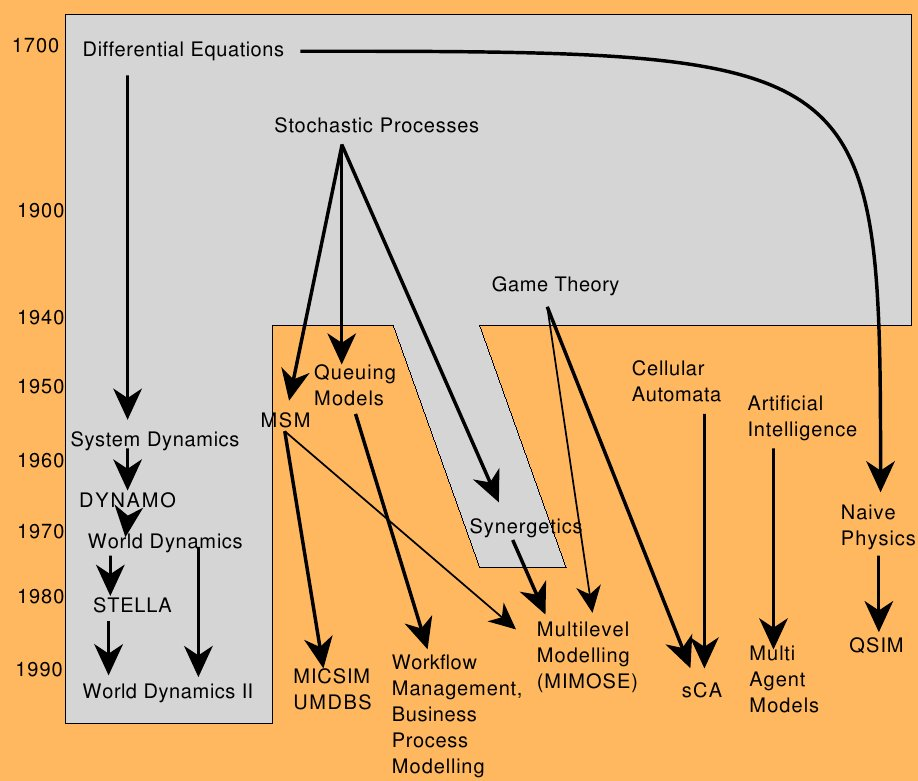
\includegraphics[width=120mm,keepaspectratio=true]{figures/Gilbert_pg21.jpg}}
\caption{The development of contemporary approaches to simulation in the social sciences (after Troitzsch )\cite{GilbertTroitzsch}}
%by Gilbert \cite{GilbertTroitzsch}}
\label{fig:SimAppGilbTro}
\end{figure}

%possible paradigms. TOASK : Explico mes que son sistemes dinamics i la resta d'opcions?????

The first paradigms to model social processes were borrowed from the fields of physics, operations research, and economics materialized as game theory. The first social concepts considered were those related to social units or subgroups and large processes. Also, due to the main use of dynamical systems and differential equations, social phenomena was modelled as a flow between different containers that represent groups or state of individuals.\\

\begin{figure}[h]
\centering
\setlength\fboxsep{0pt}
\setlength\fboxrule{0.5pt}
\fbox{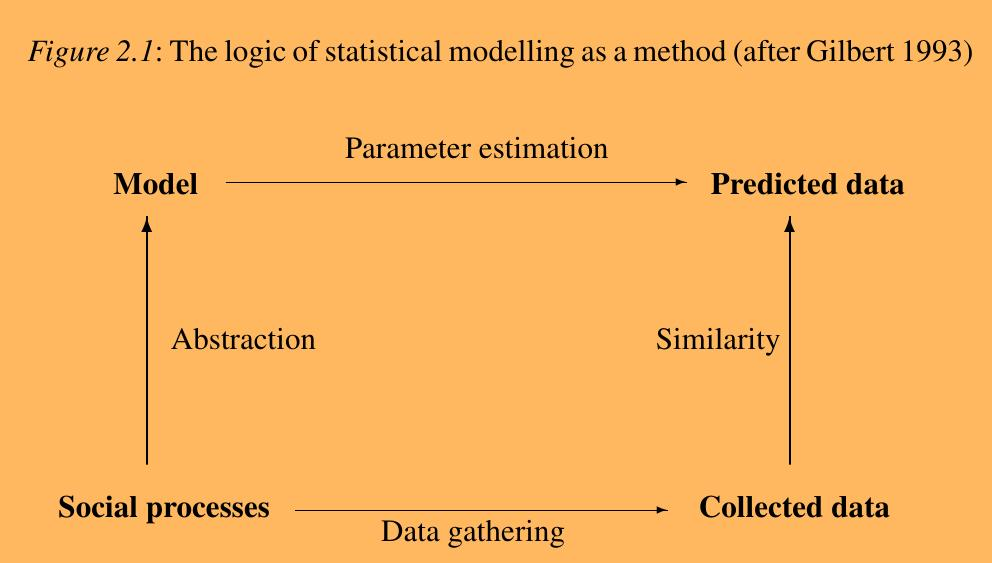
\includegraphics[width=120mm,keepaspectratio=true]{figures/statisticalModelling1.jpg}}
\caption{The logic of statistical modelling (after Gilbert 1993)\cite{GilbertTroitzsch}}
%by Gilbert \cite{GilbertTroitzsch}}
\label{fig:SimStatMod}
\end{figure}

Richer representations to cope with reality led to nonlinear specifications and the introduction of heterogeneity present in social systems making them hard to represent or analitically unsolvable, hence, the following years saw the spreading of \textbf{simulation techniques}, first AI aproximations, cellular automatas and Petri's networks that allowed a finer granularity going from the top abstract groupings infered in social theories to the individual entities.\\

Gradually social modelling began to approach computational sciences keeping its connections to mathematics and statistics. Programming languages are more expressive, less abstract than most mathematical techniques. Programs deal more easily with parallel processes and processes without a well-defined order of actions compared to math equations. There is a quite long experience on studying programs and their properties from Algorithmics, Soft Engineering, and Operating Systems. The enginering of big models benefits from these branches endowing them with the desirable properties of modularity, extendibility, the experience of combining programs to grow huge program systems, error detection and maintenance, to mention some \cite{TaberAndTimpone1996}.

\begin{figure}[h]
\centering
\setlength\fboxsep{0pt}
\setlength\fboxrule{0.5pt}
\fbox{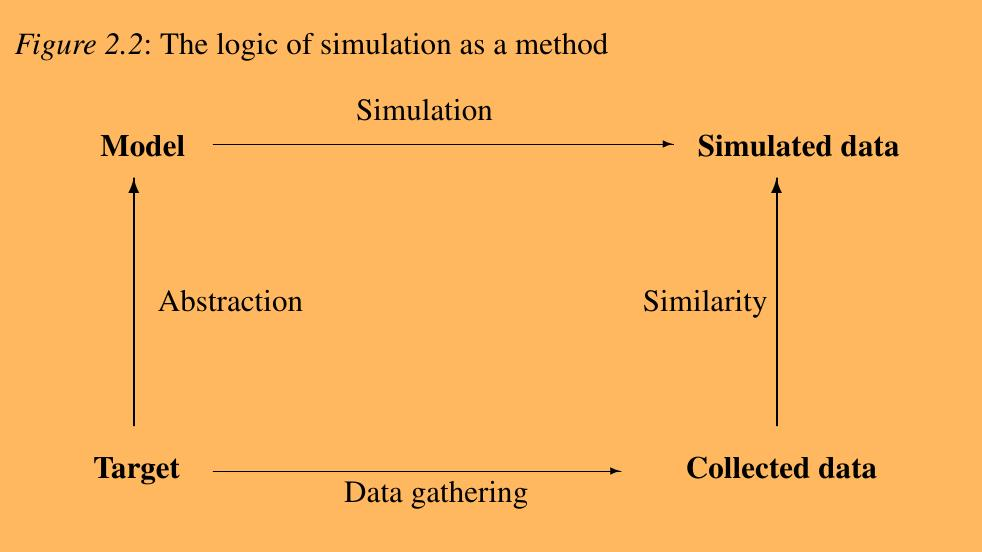
\includegraphics[width=120mm,keepaspectratio=true]{figures/simulationModelling1.jpg}}
\caption{The logic of simulation as a method (after Gilbert 1993)\cite{GilbertTroitzsch}}
%by Gilbert \cite{GilbertTroitzsch}}
\label{fig:SimLog}
\end{figure}

%non covered issues that motivate ABM, 
%TOASK separo més l'explicacio? part1: primers pseudo-agents part2:agents 100%, propietats aconseguides...
This last improvement and the use of MultiAgent Modelling in social modelling allowed to introduce the bottom layer of the hierarchy of concepts of social science, \textbf{people} and all the package of phenomena and issues associated to it. Once you are modelling a person you can work directly with personal or social relationships and their properties, arity, creation and destruction mechanisms, transitivity and interaction rules. This allows to solve models non solved before, like some cooperation, coordination and competition scenarios from game theory where several agents are involved, for instance. Also the direct interaction and feedback effects between the entities and the environment can be represented in the model. Before this step, other paradigms could not cope with the intrinsic phenomena of people interacting in a social scenario. Different issues had to be modelled, agent decission process modelling and embedding of the Rational Choice Theory, heterogeneity in the entities, bounded rationality, and complex psychology.\\ 
Modelling from a bottom-up point of view including agents will allow to be near the real causes of macroscopic large scale phenomena non predicted from the microscopic local issues. Complex systems theory calls this \textbf{emergence}. 
 
Considering specifically archeology, the introduction of modelling led to the first use of these models as emulation of reality. ABM was used to reproduce the patterns in the material samples found. This led to think ABM as a way\pdfcomment{atm: no m'agrada way} of statitistical distribution fitting. ABM models where thought as models that aproximated stochastic variables and patterns in the model. This was the scientific use of ABM. With the idea of producing more accurate explanations of the phenomena, ABM models began to be filled with more details. The objective was to approach the model to reality to obtain nearer outcomes to the data taken as reference. Those first models were designed to be a mirror of reality, and that is why some experts have been calling them Emulation Models. As it is discused by Premo \cite{Premo2010_pg33} this stalled the usability of models, first due to the difficult of interpreting the causality and processes in a simulation experiment that lead to the arising of phenomena, and second, due to the problem of \textbf{equifinality} \cite{Premo2010_EQF}.\\
The simulation of a model produces a trace of the states visited by the system. If we execute a stochastic model, the states will be conformed by the exhibited values by the model variables following some distribution. That trace is just only one from all possibles that could appear from the combinations that randomness can produce in the variables. Hence, for a single model and an initial configuration, the stochasticity can lead to many different traces although the system finishes at some atractor state or the same patterns arise. The question is, which trace must be taken into account to explain evidences found in reality? This would be an example of equifinality (figure \ref{fig:Equifinality}). There is also equifinality when given different initial conditions or assumptions on the model  and the same outcome is reached. Which is the initial escenario that produced the evidences? Due to the long time of the history trace, all initial conditions could have the same probability and data does not makes easier the discrimination. Equifinality also appears when the system exhibits sensitivity to initial conditions. Sensitivity is a typical trait of \textbf{complex systems} and it is better known as the \textbf{butterfly effect}. A small perturbation, that is considered \textbf{negligible}, in a initial condition can produce a trace with opposite conclusions to another one without that perturbation. Furthermore, due to sensitivity again, an initial condition in different runs belonging to a same simulation experiment will have usual small perturbations appearing as differences between different traces. Sensitivity to these small inner perturbations can lead to opposite outcomes in the experiment making it difficult to extract and deduce the common patterns or general behaviour we desire to check against data. It will be harder to separate noise from information. The same listed issues hold when instead considering several initial states or assumptions we consider diverse models as candidates for the explanation.

% different models can explain the outcome, which model must be chosen? -> EQF

% . y aixo es un unsustainable situaion per a extraccio espitemologica. No pots deduir una llei general, perque es inestable...

%And that is an example of equifinality. ... mention the other cases ... need to reduce detail .... another
%epistemological target and strategy -> Explor. Models ... explo mod features

\begin{figure}[h]
\centering
\setlength\fboxsep{0pt}
\setlength\fboxrule{0.5pt}
\fbox{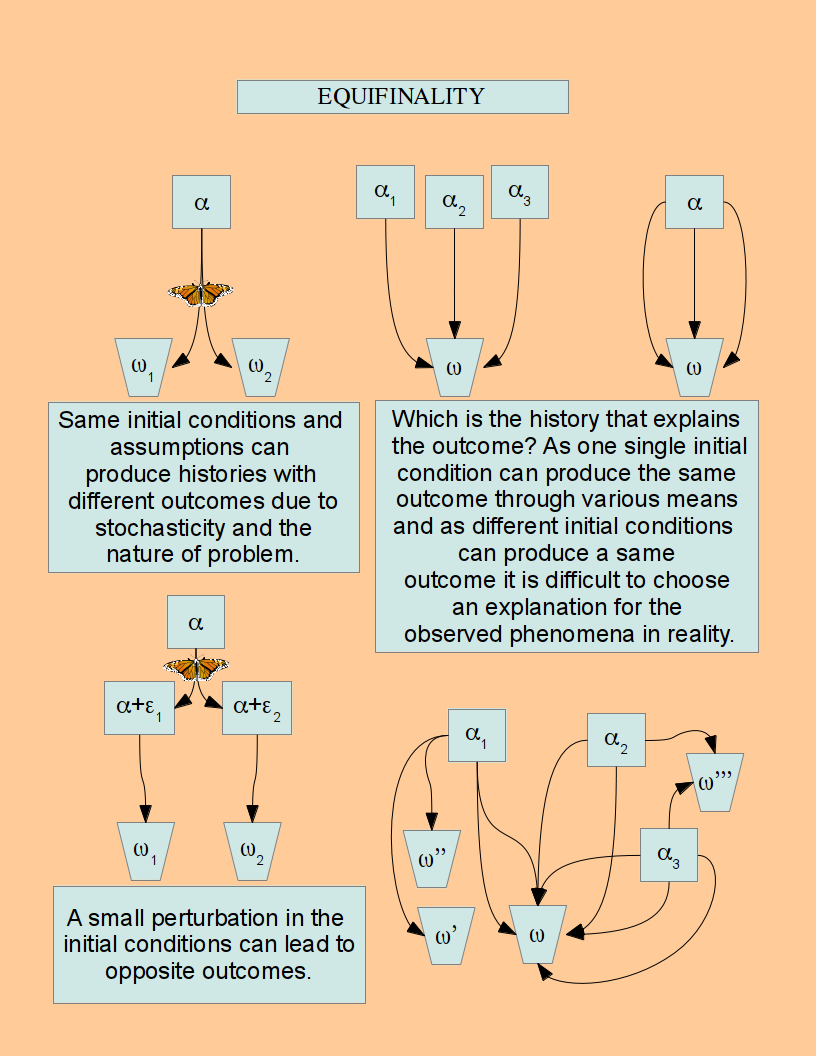
\includegraphics[keepaspectratio=true]{figures/eqf.png}}
\caption{Equifinality in stochastic simulation models. For an initial state 
	with its assumptions $\alpha$ a simulation generates a trace of states 
	that lead to a final state or set of patterns and phenomena $\omega$.}
\label{fig:Equifinality}
\end{figure}
% 

There is an alternative way of exploiting ABMs, but it implies another epistemological strategy. ABMs will be 
used as \textbf{Exploratory Models}\cite{Premo2010_EXPLOR}. Models can be simplified to the bone. This would 
keep the most essential processes related to the scientific question that motivated the simulation. As it is said 
above\ref{myPremo_simplicity}, a simple model allows a clearer insight of what is happening, and the path of 
causality between the constituents and the phenomena. Then, taking advantage of equifinality, the use of the 
model is to explore causality and tendency, how happens the connection between assumptions and parameters with 
phenomena and states. Simplicity allows to design controlled experiments and very explicit and bounded assumptions 
for hypothesis generation about the model to enhance the knowledge about processes we model from reality. Then
experiments will explore the space of parameters under sensivity to detect ranges, tendencies or configs that
produce patterns similar to or far from the empirical observations.

%generation of hypoth linked to abduction/retrodiction, Premo pg 34, last paragraph

Generation of new hypothesis and questions can be of profit for theory improvement or theory building and 
self-critcism in a loop of modelization and question-discovering feeding each other \pdfcomment{atm:cada 3 
frases hauria de posar una ref a Premo, es excessiu? fau referencia en un punt i dic q tot el que he posat ve d'alla?}. 


%When you construct a model you must think how will you use it, how will you apply it to a rational process 
%for knowledge production. 

%You must give another epistemological use to your models. Another strategy to these techniques.... Explo Models

%do not replicate evidence, but investigate processes and interaction

%ontological reductionism : MODEL({p1,p2,...p_n}) vs system

%pragmatical reductionism : MODEL(p1)+MODEL(p2)+...+MODEL(p_n) vs system


\begin{figure}[h]
\centering
\setlength\fboxsep{0pt}
\setlength\fboxrule{0.5pt}
\fbox{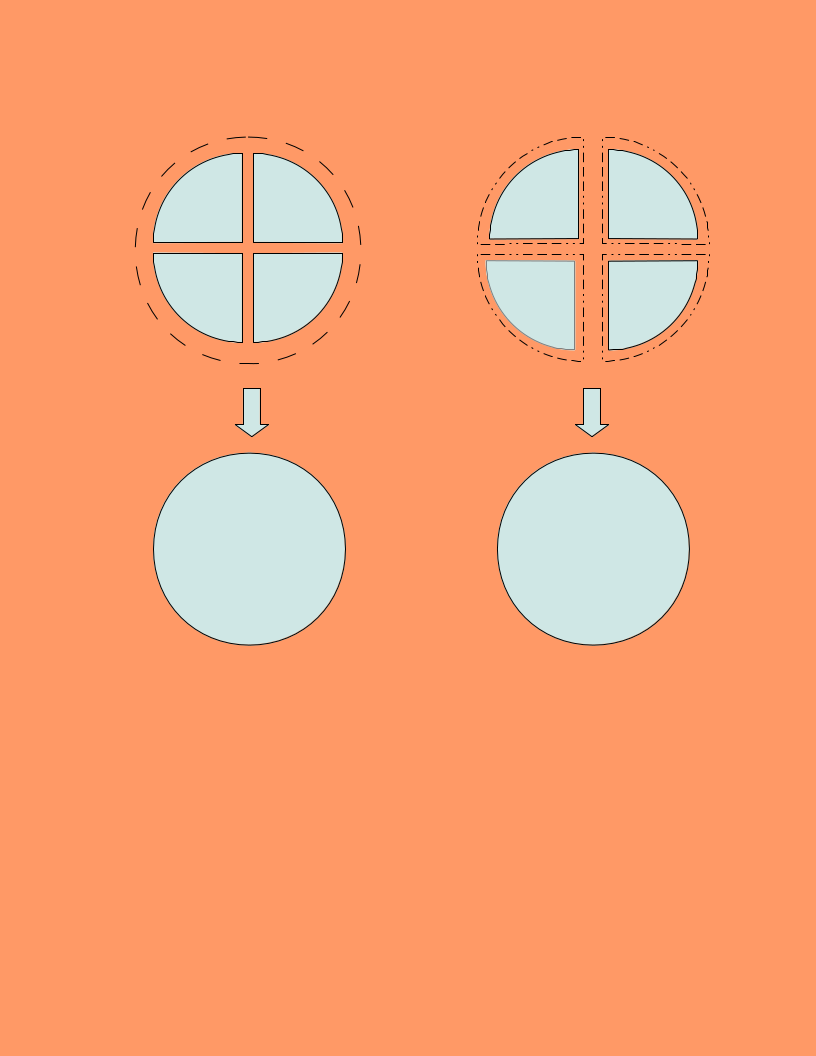
\includegraphics[keepaspectratio=true]{figures/pragmaticReduct.png}}
\caption{Ontological Reductionims vs Pragmatical Reductionism.}
\label{fig:Equifinality}
\end{figure}


 
Bound wall : EQF + obscure causality networks. We reduce detail to reach the essential processes and apply this
models to another line of thought. SImpler models -> more controlled experiments and more insight in the 
behaviour of the constituents-> exploratory of the behaviour, it is more interesting to exploit EQF and multi histories
to sample the causality space to test the initial assumptions,altres coses q miren...
The reasoning about the model outcome will be channeled to a retroductive frame.

% per on poses aixo? : ``Richer representations to cope with reality led to nonlinear specifications and the introduction of heterogeneity present in social systems''. 

Modelling methodology will be materialized through the framework of simulation technique. It will follow a series
of stages defined in simulation-based research. 

\begin{description}
\renewcommand{\labelitemi}{$\bullet$}
\renewcommand{\labelitemii}{$\cdot$}
\item [Definition of the target] A purpose for the model or a question over the target system is stated.
	\begin{description}
	\item [prediction/prognosis]
	\item [diagnosis]
	\item [theory validation / discovering]
	\item [study future possible worlds]
	\end{description}
\item [Observations] Data gathering, parameters and initial conditions retrieval from the target system using bibliography, interviews and experts' supervision.
\item [Assumptions] Relevant simplifications are considered. 
\item [Design model] Translation of the experts' conceptualizations to a formal modelling language or structure. 
\item [Computer programming] Implementation of the model.
	\begin{description}
	\item [verification] Test that the program matches the specifications and features of the formal model.
	\end{description}
\item [Run simulation] Perform the experiments.
\item [Gather results] Extract conclussions from the simulation data. 
\item [Validation] Check that the conclussions are scientifically sound and match the plausible target system behaviour. The model should behave similar to the target system under the selected features and details.
	\begin{description}
	\item [sensivity analisys] Detect variables and parameters that produce great oscilations on the simulation results.
	\end{description}
\end{description}
%%TODO GRAFIC del "cicle``

\begin{figure}[h]
\centering
\setlength\fboxsep{0pt}
\setlength\fboxrule{0.5pt}
\fbox{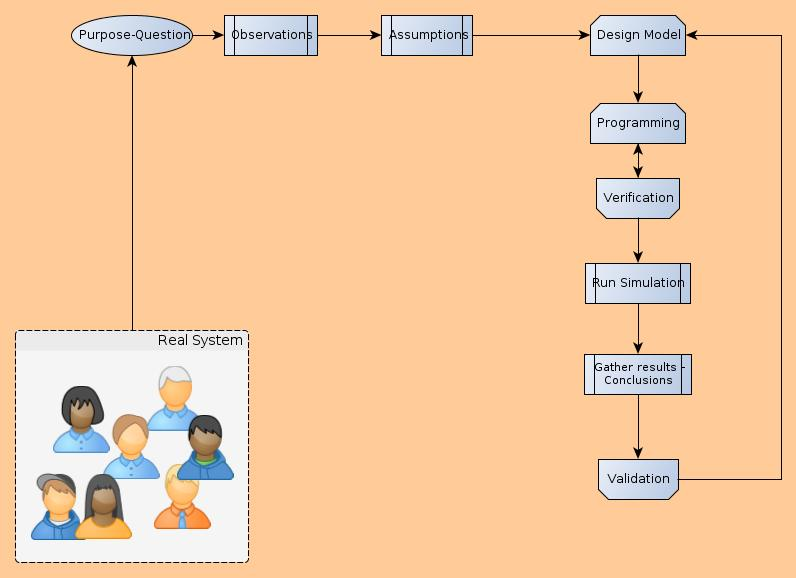
\includegraphics[width=120mm,keepaspectratio=true]{figures/simulationMethodlogy.jpg}}
\caption{Stages defined in simulation-based research \cite{RussellNorvig}}
%by Gilbert \cite{GilbertTroitzsch}}
\label{fig:SimStages}
\end{figure}


%bridge to ABM section

%%%% end content


% TOASK afegir certs apartats de l'ODD??? adaptar les descripcions dels apartats de l'ODD\\


%%%%%%%%%%%%%%%%%%%%%%%%%%
\section{Conceptual Framework}

\subsection{Multi Agent Systems} %% M.A.S.

%% aqui poses tota la part mes tecnica/teorica dels agents, a ABM ja no caldra explicar-ho
%% ABM explicara issues de modelatge i aplicacio cientifica

%% Agent System : equal agents in a shared environment
%% Multi Agent System : Heterogeneous agents.
%% TODO refina definicio 

%% definition
Multi Agent System(MAS) is an architecture for software development based on designing a solution for a problem that 
executes of a set of computational entities called agents that interact themselves in a defined environment.\\
Such entities are active decission making actors in the modelled system. The modelling lifecycle of an MAS will consider a stage where decission making processes must be identified from the system. Usually those decission making actions are carried along by more or less clear individual entities from the system. The modelling process will take the task to set the matching between these entities and the agent that will form the MAS. The concept ''agent`` condenses a set of features that will specify the modelling metaphor that an agent represents:
some enclosed set of mechanisms to be aware of the state of the system, a set of goals to accomplish and the engine to decide from a bounded perception of the world, the actions to apply on it to achieve these goals. Besides the reasoning component of the agents, MASs have a strong component of inter-agent relationship. How one agent interacts with other agents could as important or more as how it reacts to world changes.

%%bottom-up approach, reductionist way of looking at the things, we try to understand the parts\\
%%to join them from their relationship and then we try to get the big picture.

\subsubsection{Agents}

%%TODO TOASK definir nomes el necessari per a la comprensio dels ABMs? anar mes enlla i tocar features q no
%% ens son rellevants??

%%---------agents, una component que dispara la no linearitat i per tant la complexitat\\
%%---------heterogeneitat : dos \`atoms de Carboni es comporten igual en mateixes condicions, les persones no.\\

%%refine

An agent is a computer system that is capable of independent action on behalf of its user or owner,
figuring out what needs to be done to satisfy design objectives, rather than constantly being told.\cite{Wooldridge2002} An agent solves problems applying iteratively the schema of sense, decide and 
act continously. Each of the steps can add new targets to fulfill which will keep the agent exploring 
the environment and interacting with it and other agents to develop its strategies to solve the tasks 
and achieve goals.\\

Agents are \cite{WooldridgeJennings1995}:
\begin{enumerate}[i-]
 \item clearly identifiable problem solving entities with well-defined boundaries and
interfaces;
\item situated (embedded) in a particular environment—they receive inputs related to the
state of their environment through sensors and they act on the environment through
effectors;
\item designed to fulfill a specific purpose—they have particular objectives (goals) to
achieve;
\item autonomous—they have control both over their internal state and over their own
behaviour;
\item capable of exhibiting flexible problem solving behaviour in pursuit of their design
objectives—they need to be both reactive (able to respond in a timely fashion to
changes that occur in their environment) and reactive (able to act in anticipation of
future goals).
\end{enumerate}


	\begin{figure}[h]
	\centering
	\setlength\fboxsep{0pt}
	\setlength\fboxrule{0.5pt}
	\fbox{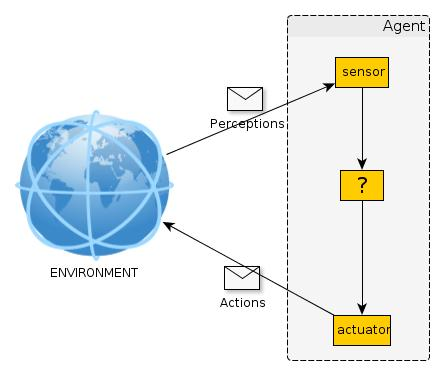
\includegraphics[width=60mm,keepaspectratio=true]{figures/agentArchitect0.jpg}}
	\caption{Agents interact with environments through sensors and actuators.}
	%by Wooldridge2002 \cite{Wooldridge2002}}
	\label{fig:AgWool}
	\end{figure}


 	\begin{algorithm}[H]
	\SetAlgoSkip{} 
	\SetAlgoLined
	initialization\;
	\While{not end}
	{
		s = read environment current state\;
		a = getAction(s)\;
		launch(a)\;
	}
	\caption{Agents basic main loop.}
	\end{algorithm}

An example of a very simple agent would be a thermostat. It samples the environment with a probe/sensor, 
checks if the temperature corresponds to the desired one. According to the measure it launches one of the two 
actions, to set the heater to ON or to OFF.\\
But we could have something as complex as an agent representing a car in a traffic simulation while drives 
from one point to another in the city. The agent would have accesible a knowledge base of traffic rules 
constraining its actions. The agent at each time step of the simulation would control the swarm of other 
vehicles to avoid collisions and would follow paths and perform actions coherent to the rules of traffic. 
The traffic rules would act as middle interface consensus of fair driving that coordinates all the cars 
and allows some prediction of the adjacent cars. The agent can be designed a step further. When congestion 
increases to a predefined threshold, which could be tuned through authomatic learning, the agent recalculates 
the route to adapt and avoid the traffic jam.\\
Intelligent agent design considers the setting of Perceptions, Actions, Goals and Environment. These
aspects form a general structure where an agent design can grow. Mentioning an example considering a 
system that simulates hunting practices from ancient cultures will show how features from the agent are 
attached to these modules in the structure(table \ref{tab:hunterAgentSetting}).\\
	\begin{table}[h]
	\centering
	\begin{tabular}{|l||l|}
		\hline
		\textbf{Perceptions} & Hunger, TerrainSlope, ReadTracks, LookForPrey.\\
		\textbf{Actions} & Eat, LightFire, Cook, ThrowArrow, Walk, Run, Stalk, Hide.\\
		\textbf{Goals} & Survive, AvoidHarm.\\
		\textbf{Environment} & Weather, Plants, Mountain, Valley, Caves, Deers, Rabbits.\\ 
		\hline
	\end{tabular}
	\caption{Setting table for a hunter agent.}
	\label{tab:hunterAgentSetting}
	\end{table}

%%TODO TOASK cal ser tant pedagogics i esmentar quins designs hi ha?
%% endow with task-solving -> reasoning -> Agent Design
%% endow with interaction managing -> society design -> MultiAgent Systems Design

%%\subsubsection{Agent Architecture Specification}

\paragraph{Agent formal description}
	
Let E be an environment with a finite set of states 
\begin{equation}
	\Omega = \{\omega_0,\omega_1,\ldots \}
\end{equation}
Each agent has available a set of actions 
\begin{equation}
	A = \{ \alpha_0, \alpha_1, \ldots \} 
\end{equation}
An action is a function that changes the state of the environment 
\begin{equation}
	\alpha_i : \Omega \longrightarrow \Omega 
\end{equation}
An agent's run is a sequence of states of the environment where the transitions were triggered 
by actions launched by the agent. Let $R$ be the set of all possible runs over $\Omega$ and $A$, and
$r^{u}$ one sequence of length $u$.
\begin{equation}
	r^{u} = ( \omega_0 , \alpha_0 , \omega_1 , \alpha_1 ,\ldots, \omega_{u-1} , \alpha_{u-1} , \omega_u )
\end{equation}
Let $R^{A}$ the sequences that end with an action 
\begin{equation}
	r^{u-1}_{A} = ( \omega_0 , \alpha_0 , \omega_1 , \alpha_1 ,\ldots, \omega_{u-1} , \alpha_{u-1} )
\end{equation}
Let $R^{\Omega}$ the sequences that end with an environment state 
\begin{equation}
	r^{u}_{\Omega} = ( \omega_0 , \alpha_0 , \omega_1 , \alpha_1 ,\ldots, \omega_{u-1} , \alpha_{u-1} , \omega_u )
\end{equation}
Actions in the run are the response of an agent $X_i$ to the states of the environment
\begin{equation}
	\forall j \in [0..u-1] : X_i(r^{j}_{\Omega}) = \alpha_j
\end{equation}
An stochastic and historic dependent environment behaviour, $\tau$, can be described as
\begin{equation}
	\tau : R^{A} \longrightarrow \wp(\Omega)
\end{equation}
A Markovian environment behaviour would be defined as
\begin{equation}
	\tau : \Omega,A \longrightarrow \wp(\Omega)
\end{equation}
and the next would hold for the runs
\begin{equation} 
	\forall i \in [0..u-1] : \tau(\omega_i, \alpha_i) = \omega_{i+1}
\end{equation}
Let's say that no end condition is described for the runs here because althought it could happen
$\tau(\omega_i, \alpha_i) = \varnothing$, many other conditions could mark the end of a run.
For instance, a run can finish because the population of agents reaches 0 due to some dying process.
A run can also stop after a finite number of transitions, or some predefined event appears.\\
\\
An agent $X_i$ retrieves information from the history of environment states to choose an action to launch
\begin{equation}
	X_i : R^{\Omega} \longrightarrow A 
\end{equation}

%%

\paragraph{Agent Main Behaviours}
\begin{description}
	\item [Autonomy] Other entities do not set the agent objectives nor decissions. With agents, 
	we give a high-level description of the delegated goal, and let the control mechanism figure
	out what to do, knowing that it will act in accordance with some built-in theory of rational 
	agency to satisfy it.

	\item [Reactivity] Response to environment stimulus or changes. A reactive agent is 
	one that maintains an ongoing interaction with its environment, and responds to changes 
	that occur in it (in time for the response to be useful). A pure reactive agent, the 
	thermostat can be formally descrived as
	\begin{equation}
		X_i : \Omega \longrightarrow A 
	\end{equation}
	\item [Proactivity] It means anticipation, taking initiative, detect oportunities. This
	could materialize in prediction of a future event an realize a set of a priori actions 
	before it occurs. For instance, if you are modelling a population of farmers and agent A1 
	sees the state of low resources of its neighbour agent A2 at the end of the season. As 
	a social action, A1 makes a pressent of food to A2 before it begins to starve or asks for
	help. We also know that this kind of action will produce stronger bonds and could have their
	pay-off in the future. But the most extended example is when you enter in a bookshop, 
	as you delay a bit in your search, a salesman appears offering its help before you ask for it.
	It could mean that the agent produces a set of actions that trigger an environment event
	that will allow the execution of an action the approaches the agent to its goals.

	\item [Social capabilities] Cooperation, coordination, negotiation, competition, and mind models.
	Some objectives are not achievable by the only means of the agent. The agent must interact
	with other entities that can produce the chain of actions to produce the changes in the
	environment needed.
	%conflict
	Agents inhabit and intearact with the environment applying actions and producing effects
	in a same medium. Goals, effects and dynamics can clash. Is it possible the appearance of
	conflict. Goals and planned trend can be contradictory for more than one agent. According
	to the model of negotiation of the agent it can try to change its plan trying to not interfere
	with the other agents, or produce a deliberate interference or ignore it and stick to its
	objectives.
	Social capabilities will cover the spectrum of comunication but also integrate the other agents
	behaviour. Some sophisticated agents include mind models to add, predict the other agents' 
	behaviour in its knowledge representation engines.
	\begin{description}
		\item [Cooperation] Cooperation is working together as a team to achieve a shared goal.
		Often prompted either by the fact that no one agent can achieve the goal alone, or that 
		cooperation will obtain a better result (e.g., get result faster). That is very easy
		exemplified with hunt parties or some families of farmers that while one member takes care
		of the plot the other takes the cattle for grazing.

		\item [Coordination] Coordination is managing the interdependencies between activities.
		For example, if there is a non-sharable resource that you want to use and I want to use, 
		then we need to coordinate.

		\item [Negotiation] Negotiation is the ability to reach agreements on matters of common 
		interest. At the appearance of conflict a solution that benefits the parts is searched.
		For example: Two farmers arrive at a piece of land good for crop growing. A possible deal: split
		the land in two.Another solution : both work on the land, but each has assigned different
		tasks. By the end of the year they divide the harvest. Typically involves offer and 
		counter-offer, with compromises made by participants.

	\end{description}

	\item [Learning] Prediction for future situations,reuse solutions,avoid past errors. The agents stores
	patterns from the history of environment changes, or other agents' actions. The patterns induce a model
	of the world or of the task to perform used by the agent for future actions. As a detail, although the 
	learning could be produced in first stages of the run to produce benefits along the life of the agent,
	it is desirable that the learning should occur along all the run to produce a real adaptation of the 
	agent. The keyword is \textbf{incremental learning}.
\end{description}

%% extra properies:Mobility,Veracity,Benevolence,Rationality,Learning/adaption.

\paragraph{Intelligent Agents Architecture}

This paragraph will show different decompositions of how an agent is structured 
and provide an answer to the question of how the sensor data and the current internal 
state of the agent determine the actions and future internal state of the agent.
The thermostat example contains an environment with a bounded and tractable number of states.
Such situations can be solved with a direct implementation setting the bijective function 
state - action with a table or with a limited number of rules.
As complexity of modelled systems grows, the number of states and possibilities become
untractable. Theres no time nor space to specify each correspondence. The agents apply different 
techniques for retrieving features and structure from the environment to proceed with the
decission process from an abstraction to the action to perform \cite{RussellNorvig}.  

\begin{description} %% we are interested in this division
	\item Reactive Architectures

The decission process in Reactive Architectures selects actions only based on the last perception retrieved
from the environment. It does not considers any subset of past perceptions. Reactive Architectures encompass  
the Simple Reflex Agents.

		\begin{figure}[h]
		\centering
		\setlength\fboxsep{0pt}
		\setlength\fboxrule{0.5pt}
		\fbox{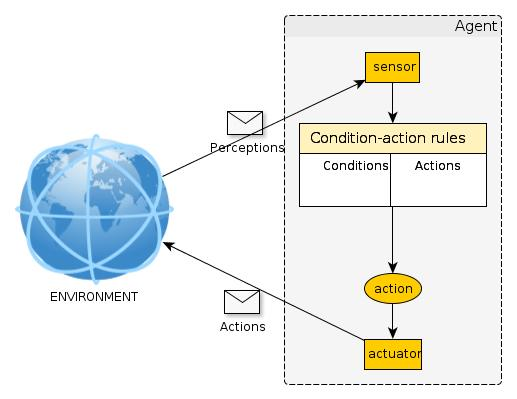
\includegraphics[width=80mm,keepaspectratio=true]{figures/SimpleReflexArchitect0.jpg}}
		\caption{Simple Reflex Agent Architecture}
		%by RussellNorvig \cite{RussellNorvig}}
		\label{fig:SimpleReflexArchitect0_label}
		\end{figure}

A change in the environment provokes a response from the agent. When changes and deliberations in agent are
only motivated by an event in the environment, the agent is pure reactive.\\
	
		\begin{algorithm}[h]
		\SetAlgoLined
		\SetKwData{rules}{rules}\SetKwData{rule}{rule}\SetKwData{I}{I}
		\SetKwFunction{getNextPercept}{getNextPercept}\SetKwFunction{brf}{brf}\SetKwFunction{options}{options}\SetKwFunction{filter}{filter}\SetKwFunction{plan}{plan}\SetKwFunction{execute}{execute}
		\BlankLine
		\While {true}{
			$\sigma$ $\gets$ getNextPercept()\;
			$rule$ $\gets$ ruleMatch($rules$, $\sigma$)\;
			$\alpha$ $\gets$ ruleAction($rule$)\;
			execute($\alpha$)\;
		}
		\caption{Simple Reflex Agent main loop}
		\end{algorithm}

	\begin{itemize}
		%%refine \item With Internal state vs without internal state

		\item Cognitive Maps
		\item State Transition Machines %% TODO mira exemple

		\begin{figure}[h]
		\centering
		\setlength\fboxsep{0pt}
		\setlength\fboxrule{0.5pt}
		\fbox{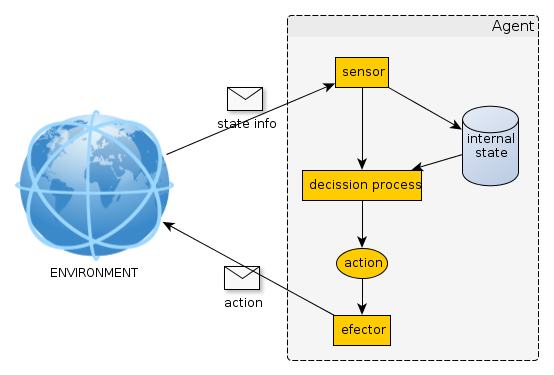
\includegraphics[width=80mm,keepaspectratio=true]{figures/agentArchitect1.png}}
		\caption{State Machine Reactive Agent Architecture}
		%by Wooldridge2002 \cite{Wooldridge2002}}
		\label{fig:StateMachine}
		\end{figure}

		\item if-then rules
	\end{itemize}
	
	\item Deliberative Architectures

	A deliberative agent uses symbolic reasoning to deduce the action to launch. The deliberative agent
	contains explicitly the goal that steers its behaviour. Deliberation is done through an internal formal 
	representation of the state of the world, the state of the agent and other information retrieved by
	it. A logic engine will produce deductions from the facts stored in the agent memory, the knowledge
	base. The perceptions from the environment become facts to add to the internal representation of
	the environment. From this internal world model the agent can deduce trends for prediction besides
	the next action to launch. A state of the environment or of the agent is specified. The agent must find 
	the way to fulfill this within his reach of perceptions and actions. Desirable situations are seeked, 
	called goals, that is environment states or agent states. 

	Given some systems or situations, goals are non achievable from a single action execution. The agent 
	must apply search and planning techniques to conform a plan that will satisfy, after a limited number of 
	steps, the desired goal.

	Goals could be a design feature of the agent, for instance \textbf{survive} \& \textbf{reproduce}, or could 
	be set dynamically in runtime by conditions in the environment or through user commandment.

	\begin{description} 
		\item [Logic] Deliberative agents will use assert clauses and structures to represent facts in 
		a logic of some level, CP0, CP1. Each new change in the knowledge base will allow to deduce
		new facts from the status of the system to check againts the goals and other issues the agent
		is considering to produce an action coherent with the planning and the mechanics of the environment
		to fulfill a new step to get nearer to the goals.
		%%TODO dibuix de la taula i els objectes mes la representacio interna : on(), above(),under()
		The agent will use its knowledge base as a theory of the world and things plus the dynamic facts
		that represent the volatile states.\\
		Let $\rho$ be a theory of the world. Depending on the architecture this can be a set of rules,
		or a learned structure along the run.\\ 
		If $\Gamma$ is a description for the current state of the world. $A$ the set of possible actions 
		\{$\alpha_1$, $\alpha_2$, $\alpha_3$, \ldots\}. And $\Gamma \vdash_{\rho} \Phi$ stands for a succesful 
		prove that $\Phi$ is deduced from the knowledge base $\Gamma$ using theory $\rho$. The Deliberative 
		agent will choose actions according to a schema like that:

		\begin{algorithm}[H]
		\ForAll{$\alpha \in A$}{	
			\If{$\Gamma \vdash_{\rho} doAction(\alpha)$}{
				\Return $\alpha$;
			}
		}

		\ForAll{$\alpha \in A$}{	
			\If{$\Gamma \nvdash_{\rho} \neg doAction(\alpha)$}{
				\Return $\alpha$;
			}
		}
		\Return null;
		\end{algorithm}

		Asserts from Logic will be used to state the facts that are true from environment
		and the other agents.
		% Knowledge representation. Solvers : Resolution, Forward/Backward chaining
		
		\item [BDI] BDI stands for Belief-Desire-Intention. Yoav Shoham introduced “agent-oriented 
		programming” in 1990 \cite{Shoham1990}:“new programming paradigm, based on a societal view of
		computation”. The key idea is about directly programming agents in terms of \textbf{intentional}
		notions like belief, commitment, and intention.	Beliefs are used to model the state of the world.
		Desire allows the selection of possible states of the world and preferences. Intentions are 
		compromises to achieve a given state, they are the commitment of the agent.

		BDI belongs to a overloaded kind of logics called modal logics which add meta language operators to
		the facts to alter with some nuance the meaning or the semantic interpretation of the fact.
		For instance, let $\phi$ be a fact that could represent ``deer is in the wood''. Indeed it is true
		for the example. Our agent has not seen it and only has some clue that the deer is in the 
		wood; so the agent states $\Box_B \phi$, with an operator $\Box_B$ to indicate ``I believe the 
		deer is in the wood''. The memory of the agent will contain also the facts below
		  \begin{description}
		    \item[$\theta$] = ``I am hungry''.
		    \item[$\eta$] = ``I go hunting''.
		    \item [$\Box_D \eta$] = ``I have Desire for going hunting''.
		    \item [$\Box_I \eta$] = ``I have Intention for going hunting''.
		  \end{description}
		Some of these entail from other. They are governed by the next rules from the knowledge base
		\begin{itemize}
		\item myState(HUNGRY) 
			$\rightarrow$ $\Box_D$ doAction(HUNT)
		\item $\Box_D$ doAction(HUNT) $\wedge$ $\Box_B$ entityAtPlace($x$,$y$) $\wedge$ edible($x$)\\ 
			$\rightarrow$ $\Box_I$ doAction(HUNT)
		\item $\Box_I$ doAction(HUNT) $\wedge$ $\Box_B$ entityAtPlace($x$,$y$) $\wedge$ edible($x$)\\ 
			$\rightarrow$ doAction(go, $y$)
		\item entityAtPlace(MYSELF,$p$) $\wedge$ $\Box_I$ doAction(HUNT) $\wedge$ entityAtPlace($x$,$y$) $\wedge$ edible($x$) $\wedge$ distance($p$,$y$) $\leq$ HUNTDISTANCE	
			$\rightarrow$ doAction(HUNT,$x$)
		\item doAction($a$,$x$) $\rightarrow$ launchAction($a$($x$))
		\end{itemize}

		This rules would carry the agent to satisfy the goal of feeding going through the goal of going where the
		prey is, and see that it is indeed there where the agent believed.

		Programming agents this way allows a deeper description of the dynamics around the goals an agent 
		self-imposes and also an easier way for the agent to reason about the other agents. This last point
		is crucial for a better integration of the social dynamics in the planning of goal achieving. The agent
		can construct through facts of Believing, Desire and Intention a mind model of the other models taking
		into account their BDI intentions and adapting to them to cooperate or compete. 

		Continuing the example, the agent would be inmersed in social deliberations after retrieving from the
		world facts like $\Box_{I}^i \eta$ that stand for ``Agent $i$ has the Intention of hunting''. The 
		interaction of all these facts, entityAtPlace(MYSELF,P), entityAtPlace($i$, P) will make deduce to the
		MYSELF agent somekind of communication protocol with agent $i$ to solve the conflict. Because they could 
		end to hunting the same deer, before they would launch their HUNT action, they must reach a consensus about
		what to do each other. 

		Schema for BDI	

		\begin{algorithm}[H]
		\SetAlgoLined
		\SetKwData{B}{B}\SetKwData{D}{D}\SetKwData{I}{I}
		\SetKwFunction{getNextPercept}{getNextPercept}\SetKwFunction{brf}{brf}\SetKwFunction{options}{options}\SetKwFunction{filter}{filter}\SetKwFunction{plan}{plan}\SetKwFunction{execute}{execute}
		\BlankLine
		$B \gets B_0$\;
		$I \gets I_0$\;
		\While {true}{
			$\delta$ $\gets$ getNextPercept()\;
			$B$ $\gets$ brf($B$, $\delta$)\;
			$D$ $\gets$ options($B$, $I$)\;
			$I$ $\gets$ filter($B$, $D$, $I$)\;
			$\pi$ $\gets$ plan($B$, $I$)\;
			execute($\pi$)\;
		}
		\caption{BDI main loop}
		\end{algorithm}

		%other issues about BDI : planning of actions to fulfill intentions, and commitment management

		%TODO add the second algorithm?

		\item[Utility based]

		Goal-based models are a dycothomic approach that rely on bivalued logics. A goal is considered
		achievable or not achievable, an agent is commited to a goal or is not commited to that goal. But
		many fields have shown things usually work in a fuzzy manner or probabilistically or with multivalued
		assignations. Mentioning some example, robot soccers. In a match, eventually, you could pass the 
		ball to a partner or try to score. If you launch the action “pass” things will happen different 
		from launching action “score” but a priori you cannot predict which will be of more help. And if 
		you stop to think about it the opponent will steal the ball from you. Another example, a fire
		simulation. There are many escape routes; when a route is saturated due to congestion, people 
		have a variable internal timeout wait time to leave the route and try another one. There is also 
		fuzzy phenomena in auctions; auction agents have to decide wheter raise the ``bet'' or leave.

		%TODO arrange
		An agent under these circumstances will find a set of available goals where each one produce a
		different benefit for the agent itself. The goals, the states of agent and environment must be 
		weighted in function of probability of success, or benefit for the agent. Also, there is some related
		optimization trend or related likelihood of achieving positive results. 

		%%Uncertainty(chap13 Russell... maybe ch16)
		A pure logical agent can find a cul-de-sac on its deductions if the possible contingencies overcome
		the reasoning to deduce the actions to fulfill the goal. These issues are what is called
		\textbf{uncertainty}. Uncertainty is the term used when there are many solutions that lead to the
		goal or if the goal is something not sure to be achieved and the agent faces a choice with no 
		success ensured. 

		For instance, considering a hunter agent in a social simulation of ancient societies, a hunt action
		can be affected by many issues. First you must make a guess about where the preys are. Once you 
		begin the hunting session many things could happen: a weather incident that changes prey grace
		behaviour, other hunters appear to hunt the preys, or dangerous roaming predators. The pure bivalued
		logic agent cannot predict the setbacks so cannot deduce the sucess of the action, and the hunt 
		action will not be launched leading to starvation. If all the logical paths towards the achievement 
		of the goal are troubled by contingencies, the agent could fall in a loop of inactivity.\\ 
		When perfect solution is perhaps non achievable, the agent should be allowed to satisfy the goals
		through a non perfect solution. The decission engine should be changed to accept failable solutions 
		for its goal seeking. Another hunt area should be eligible in the decission process. But maybe,
		although the other area is free of contingencies, it cannot offer a good outcome because is almost
		dessertic. Someway the agent should express a \textbf{preference} and deduce the action planning
		according to it. Preference over the outcomes of and action in the goal seeking activities of the 
		agent encompass the modelling of success probability and benefit quantification. A particular outcome
		should be the fact that the hunter returned home without getting injured and a certain amount of 
		Kg. of meat. 

		\textbf{Utility theory} is used to represent and reason with preferences. Utility theory says that
		every state has a degree of usefulness, or utility, to an agent and that the agent will prefer 
		states with higher utility \cite{RussellNorvig}. Preference and similar issues are modelled through
		\textbf{utility functions}. 
			\begin{equation}
			 u\ :\ E \rightarrow \ \mathbb{R}
			\end{equation}
		Utility functions map desired states to a quantitative dimension, a scoring. Utility ponderation 
		allows to break ties in sub-goal selection. Utility functions will give extra heuristic information
		about the likelihood achieving a goal. If the hunter agent has acces to two areas of hunting, $valley$
		and $wood$ and is more likely to find dangerous predators in the $wood$ although the same preys can 
		be found on both areas, the utility function would assign greater utility to the $valley$. Utility
 		provides a way in which the likelihood of success can be weighted against the importance of the goals.\\
		Preferences, as expressed with utility functions, are combined with probabilities in the general 
		theory of rational decisions called \textbf{decision theory}: \cite{RussellNorvig}
			\begin{equation}
			Decision\ theory = probability\ theory\ +\ utility\ theory .
			\end{equation}

		Utility-based agents are rational and follow the principle of \textbf{Maximum Expected Utility (MEU)}: 
		\textit{An agent is \textbf{rational} if and only if it chooses the action that yields the highest
		expected utility, averaged over all the possible outcomes of the action.}\cite{RussellNorvig}.

		%\item[Utility and Planning]

		%utility functions applied to runs... 
		%%TODO (Explicar-ho? o es fa al capitol del MDP)

	\end{description}


	%\item Hybrid Architectures 
	%say you can mix everything
		
\end{description}


%%TODO TOASK Differences between Agents & Expert Systems pg17
%% why did we choose agents? why not embed and ExpSyst in our agents?

%%TODO TOASK BDIs? not decided yet. Responc aixo a la part d'agents dins l'ABM?


%%%%%%%%%%%%%%%%%%%%%%%%%%%%%%%
\begin{description} 
	\item [Environment Features]
	\item [Accessible vs Inaccessible] An accessible environment is one in which the agent
		can obtain complete, accurate, up-to-date information about the environment’s state.
		Most moderately complex environments (including, for example, the everyday physical 
		world) are inaccessible.\\
		The more accessible an environment is, the simpler it is to build agents to operate in it.
		Accuracy and completeness about information retrieved is key to decission making.
		All the missing stretch must be supplied with uncertainty managing techniques.
	\item [Deterministic vs non-Deterministic] As we have already mentioned, a deterministic
		environment is one in which any action has a single guaranteed effect — there is no 
		uncertainty about the state that will result from performing an action.
		The physical world can to all intents and purposes be regarded as non-deterministic.
		Non-deterministic environments present greater problems for the agent designer.
	\item [Episodic vs non-Episodic] In an episodic environment, the performance of an
		agent is dependent on a number of discrete episodes, with no link between the performance
		of an agent in different scenarios. Episodic environments are simpler from the agent
		developer’s perspective because the agent can decide what action to perform based only 
		on the current episode — it need not reason about the interactions between this and future 
		episodes.
	\item [Static vs Dynamic] A static environment is one that can be assumed to remain unchanged 
		except by the performance of actions by the agent. A dynamic environment is one that has 
		other processes operating on it, and which hence changes in ways beyond the agent’s control.
		The physical world is a highly dynamic environment.
	\item [Discrete vs Continuous] An environment is discrete if there are a fixed, finite
		number of actions and percepts in it. Russell and Norvig give a chess game as 
		an example of a discrete environment, and taxi driving as an example of a continuous one.
\end{description}

	\begin{table}[h]
	\centering
	\begin{tabular}{||l|l|l|l|l|l|l|l||}
		\hline
		\hline
		\textbf{Task} \textbf{Environment} & \textbf{Observable} & \textbf{Deterministic} & \textbf{Episodic} & \textbf{Static} & \textbf{Discrete} & \textbf{Agents}\\
		\hline
		Crossword puzzle 	& Fully & Deterministic & Sequential & Static & Discrete & Single	\\ \hline
		Chess with a clock	& Fully & Strategic     & Sequential & Semi   & Discrete & Multi	\\ \hline
		Poker			& Partially & Stochastic & Sequential & Static & Discrete & Multi	\\ \hline
		Backgammon		& Fully & Stochastic    & Sequential & Static & Discrete & Multi	\\ \hline
		Taxi driving		& Partially & Stochastic & Sequential & Dynamic & Continuons & Multi	\\ \hline
		Medical diagnosis	& Partially & Stochastic & Sequential & Dynamic & Continuous & Single	\\ \hline
		Image-analysis		& Fully	& Deterministic & Episodic & Semi & Continuous & Single 	\\ \hline
		Part-picking robot	& Partially & Stochastic & Episodic & Dynamic & Continuous & Single	\\ \hline
		Refinery controller	& Partially & Stochastic & Sequential & Dynamic & Continuous & Single	\\ \hline
		Interactive English tutor & Partially & Stochastic & Sequential & Dynamic & Discrete & Multi	\\ \hline
		\hline
	\end{tabular}
	\caption{Examples of task environments and their characteristics.}
	\label{tab:EvironmentCharactExamples}
	\end{table}

%%%%%%%%%%%%%%%%%%%%%%%%%%
%TODO quan parlis de les platforms, FIPA &Co, justifica que anem amb Pandora+ODD. Per paralelisme a MN?
%%%%%%%%%%%%%%%%%%%%%%%%%%


%Features:
%\\
%		  agents ( els features isolats )
%		    goal planning/seeking
%		    reasoning
%		    adaptation
%		    decission making
%		  social interaction
%		  emergence
%\\		    
%		  bottom-up modelization
%		    identify reasoning/deciding units : what will become agents
%		    identify agents' relationships. 
%\\
%		  natural correspondence/matching of identified entities in social systems vs 
%		  agents in the ABMs theoretical framework
%\\
%		  temporal correlation - histeresis
%\\
%%%%%%%%%%%%%%%

\subsection{Complex Systems}

Complexity is a discipline that studies systems that cannot be studied through the analisys of its
parts and the simple composition of those analisys. Usually, \textbf{reductionism} has coped with complicated systems
where the supression of constituents does not change the main trend of its behaviour, and it is used to
work with simplified questions. Let's think for instance in a car which more or less keeps running although 
you remove its seats, the doors, and the lights, to mention some. That is what could be called a complicated 
system \cite{MillerPage2007}.
There are systems where the interrelationship is so rich that supression of one part dismembers all the coherence
of the system. Taking again the car exemple, if we think about the engine, the suppression of a most tiny
gear will change the things, everything will stop. Historically, those systems have been an issue that was 
of concern to many disciplines, Economics, Physics and Biological sciences, that gave arise through an
interdisciplinary effort to complexity science \footnote{here we are not talking about the computational
concept of algorithm complexity.}  \cite{MelanieMitchell2009}. 
Complex science tries to find out how the interactions of a set of constituents build a system that exhibits 
adaptive traits, descentralized organization, and macroscale behaviour patterns.\\

One of the most known systems studied by its complexity are ant colonies. The colony is formed by a limited range
of roles, a queen, soldiers and workers/explorers. Each role exhibits a limited spectrum of behaviours activated by pheromones or stimulus from the environment. Soldiers attack anything that moves non impregnated by the odor of the nest. Unloaded workers follow explorer's pheromons. When food is found a worker returns home. Dead bodies or garbage found are put near other garbage, generating dump patterns. More or less this is the program of ants. And this executed by a huge amount of ants produces an ant colony that manages food resources, reproduction and care, defense and many
other adaptations to the wild life in the forest. It can loose part of its population, can balance workload, a same specific individual group of ants is not needed for an especific task. The colony is ductile, malleable. The ant 
colony acts has a whole with very rich global behaviours. That is a complex system.\\

\begin{figure}[h]
\centering
\setlength\fboxsep{0pt}
\setlength\fboxrule{0.5pt}
\fbox{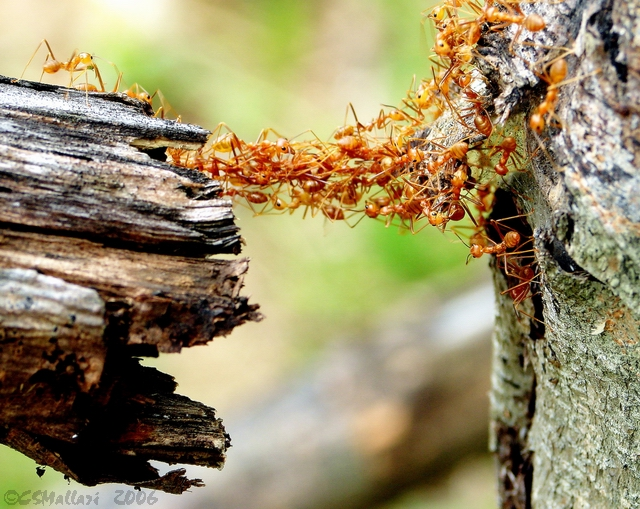
\includegraphics[width=60mm,keepaspectratio=true]{figures/ant_1.jpg}}
\caption{ Ant explorers building a bridge to overcome obstacles.}
\label{fig:ants_1}
\end{figure}


%TODO exemples : swarm, ecosystems, weather,Belousov-Zhabotinsky reaction, real economic systems, markets
%TODO game of life, we give the pressence of entitty to patterns arising from cell behaviour.

Researchers observed that woods under a fire dissappear at different rates not completely dependent to the intensity
of the focus, nor the climatic conditions. It was observed that under some tree topologies and certain wood
density a small change in the number of trees would mean sometimes the complete combustion of all the wood, and
other times the wood would only burn in a small controlled area. This topology dependant condition is called
\textbf{percolation}. It arises from the spatial relationship between the trees. Considering an ideal situation
where topology protects the wood from percolation appearance, slight changes in some trees distribution will make
them sensible to fire, but the rest of the wood will not burn. These conditions are an example of robustness
in complex systems. But enough changes will collapse it.\\
The strong relationships that give arise to the complex phenomena act as the glue that holds the system, it gives
reason to the system existence.\\ 
Percolation was not discovered studying one tree. It was detected taking into account the whole of the wood and the feedback versus the individual trees.\\

\begin{figure}[h!]
\centering
\setlength\fboxsep{0pt}
\setlength\fboxrule{0.5pt}
\fbox{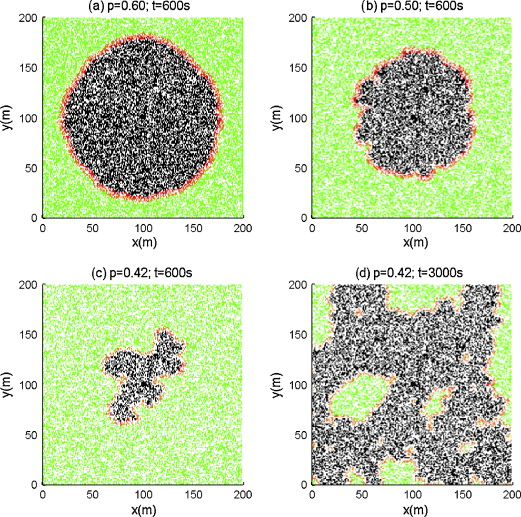
\includegraphics[width=30mm,keepaspectratio=true]{figures/percolation_1.jpg}}
\caption{ Percolation phenomena in fire spreading.}
\label{fig:percolation_1}
\end{figure}

Indeed we observe that there is a system due to the pressence of the macro phenomena. It is the evidence that
something is happening there that relates the constituents.\\

\begin{figure}[h]
\centering
\setlength\fboxsep{0pt}
\setlength\fboxrule{0.5pt}
\fbox{
\includegraphics[width=40mm,keepaspectratio=true]{figures/dictyo_2.jpg}}
\caption{ Development of spiral waves after hydrodynamic breaking of a concentric wave (Zhabotinsky and Zaikin, 1971).}
\label{fig:ZhaboZaikin_1}
\end{figure}


%TODO
%Just as an anecdotic remark, the word ``complex'' comes from the latin word ``plectere'' which means ``to weave'', ``to enwine''.

%TODO exemples : swarm, ecosystems, weather,Belousov-Zhabotinsky reaction, real economic systems, markets
%TODO game of life, we give the pressence of entitty to patterns arising from cell behaviour.
%TODO we see a shape move, form give life to a macro entity, and we observe a lifecycle of operations :
%TODO space translation, shape transformation, appearance, disappearance

%TODO Complex : emergence, self organizing, adaptive, descentralized 

Just to give a compact definition from Melanie Mitchel \cite{MelanieMitchell2009}, a complex system is a system in
which large networks of components with no central control and simple rules of operation give rise to complex collective behaviour, sophisticated information processing, and adaptation via learning or evolution. Sumarizing, a complex system exhibits nontrivial emergent and self-organizing behaviors.

%exemple -> analitzar-lo i posar de manifest la complexitat ???
% and then state what comes next:
The laws that describe its behaviour are qualitatively different from those that govern its individual units.
The advances of computational techniques for scientific discovering is changing the way we confront the models 
and the manipulation of these issues. Computers have allowed new ways of learning about them. Computational techniques 
allow the modelling of many constituents and its relationships, how they assemble to a whole system. It allows us 
to understand and play with the experimental manipulation of the behaviour in a easier way. Computers not only help 
us in studying the surface of the behavioral phenomena but also the internals of complex systems giving insight 
to our explanations and deductions. Besides, computational experimentation has the advantage of controlling the trace 
and generating rich databases of events for posterior analyses \cite{Vicsek2002}.

%TODO ara lligues Complex amb Emergence i pots passar al següent punt
Complex behaviour is tied to a non central global decission process. But, on the other hand, the emerged pattern is
something that does not belongs to a identifiable constituent. It is build from the descentralized dynamic of all 
the constituents. That feature is called \textbf{emergence}.

\subsection{Emergence}


%Emergence is „the arising of novel and coherent structures, patterns and properties during the process of self-organization in complex systems." (Corning, 2002; Goldstein, 1999)

Emergence is a phenomenon where aggregation of individual and local behaviours are the direct cause
of a higher level pattern or global behaviour. Emergence is one of the key concepts from Complexity 
that is studied in Social Simulation. Indeed, emergence is one of the main features exhibited by 
complex systems.\cite{MillerPage2007}
%TODO elabora. Emergence es un key concept

Although we can give features and descriptions, emergence cannot be fully specified due to the vague 
concepts of ``surprising'' and non deducibility \cite{Holland1997} . But some signals can 
be enumerated to circle the concept of emergence. 

A phenomenon will be considered emergent when it is repeatable and surprising, non deducible from lower 
level rules and the relationships of basic constituents of the system.
Emergence cannot be predicted, given our current means, from only the constituents and their addition, 
following the reverse way of reductionism. Reductionism is one of paradigms of science. A system is observed
to detect differentiated parts. Then each part is analized to extract its behaviour. Reductionism states
that the behaviour of the system can be understood from the constituents specifications plus a simple or 
direct aggregation step. This idea can be applied recursively on the same constituents till some atomic element
considered the bottom of the process. The thing is that due to nonlinear relationships, following the inverse
path to reconstruct a sense for the whole system is practically impossible.\\

Even a small and simple set of rules can make a dynamic system generate emergent phenomena. 
If these rules induce non linear relationships the proportion of a perturbation in the system will not 
be paired with the response of it. To use an uninventive example, nonlinear emergence occurs when someone 
\textbf{calmly} says “fire” in a crowded room and produces \textbf{explosive} panic. Unpredictable results 
arise from constituents interactions. It is here where emergence can appear. When a pattern is recognizable 
and repeats usually along experiments, is plausible to be considered emergent \cite{Holland1997}.\\  

%\begin{figure}[h]
%\centering
%\setlength\fboxsep{0pt}
%\setlength\fboxrule{0.5pt}
%\fbox{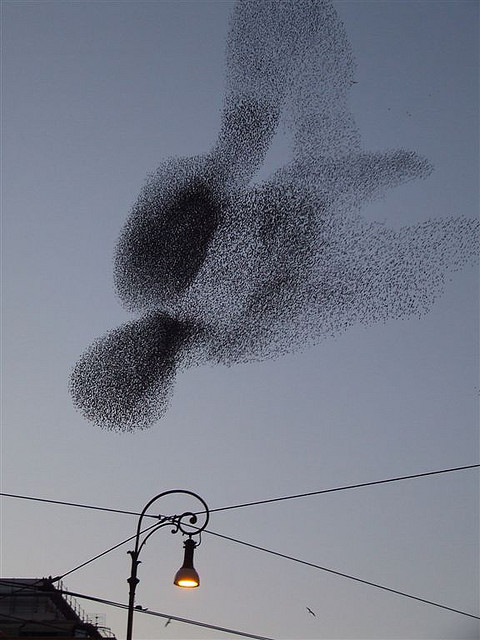
\includegraphics[width=60mm,keepaspectratio=true]{figures/swarm1.jpg}}
%\caption{ A swarm of birds flying avoiding clashes and generating patterns in the air that sometimes defend them from %predators.}
%\label{fig:swarm_1}
%\end{figure}

%\begin{figure}[h]
%\centering
%\setlength\fboxsep{0pt}
%\setlength\fboxrule{0.5pt}
%\fbox{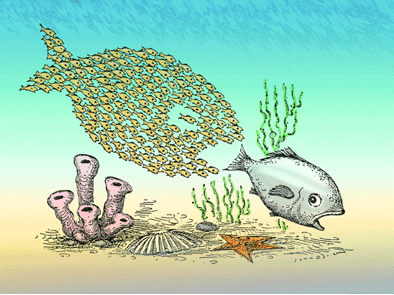
\includegraphics[width=60mm,keepaspectratio=true]{figures/emergence_1.png}}
%\caption{ Swarms of fishes generating patterns in water sometimes defend them from predators.}
%\label{fig:emergence_1}
%\end{figure}

	\begin{table}[h]
	\centering
	\begin{tabular}{|c|c|}
		\hline
		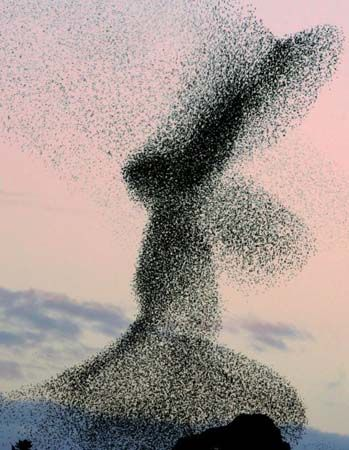
\includegraphics[width=60mm,keepaspectratio=true]{figures/swarm2.jpg}
		&
		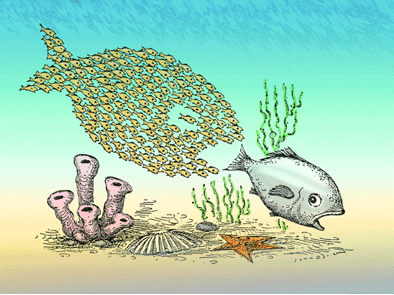
\includegraphics[width=60mm,keepaspectratio=true]{figures/emergence_1.png}\\
		\hline
	\end{tabular}
	\caption{Emergence of swarm patterns from the interaction of many moving actors.}
	\label{tab:tableSwarm}
	\end{table}


%TODO : la sorpresa que es demana sempre es sorpresa, no cansa : on surt?


There is potential for emergent phenomena, i.e., when: 
\begin{itemize}
 \item Agent behaviour is non linear ( weight sum of variables), or is expressed with discontinuities, if-then rules in a categorical framework or in discrete non continous manner.
 \item Under memory phenomena, path-dependence, and hysteresis, non-markovian behavior, or temporal correlations, including learning and adaptation. 
 \item Heterogeneous interactions between agents.
 \item When there is unstability to perturbations although the system could be defined linearly.
\end{itemize}


\subsection{Evolution}
%TODO\underline{	Darwinisme : survival of the fittest.
%		Ingredient afegit per a testejar l'adaptabilitat i el fitness de les dues estrategies : HG vs AP
%		Dins el mark evolutiu establirem la competencia entre les dues estrategies : qui pugui tenir una
%		millor supervivencia del seu offspring perpetuara  la seva estrategia (ADN)
%		}

Evolution theory is the result of observations made by Charles Darwin in his trips to Galapagos Islands and 
study of native species of finche birds. Darwin proposed that the varieties and specializations of observed
species was imposed by the topology of the island and the local conditions of each one. The theory arised from
the following points in conjunction of the observations. He based his deductions on
the next hypothesis:
\begin{itemize}
	\item Gradual change over long periods can produce very large effects.
	\item Population growth combined with limited resources creates a struggle for
	existence. 
	\item Collections of individuals acting in self-interested ways produce
	global benefit. 
	\item Life seems to allow almost infinite variation, and a species’
	particular traits seem designed for the very environment in which the species
	lives. 
	\item Species branch out from common ancestors.
\end{itemize}

Darwin called \textbf{Evolution by Natural Selection} to the improvement by mutation and competition process 
where individual beings produce offspring at a rate greater of the survival rate ( otherwise they 
would extinct). The offspring is almost equal to the parents except from slight variations. At 
some point the population will saturate the niche and they will compete for the resources.
The more adapted individuals are considered those who will satisfy their resource needs and
have higher reproduction success. This will imply that a great number of offspring that inherited
features from their successful parents will populate the environment. These traits will persist
through the time from generation to generation. This would explain why individuals are as they are
and not other way. Adaptation comes from the small perturbations or changes between parents and
offspring. This is an open door to the appearance of an improved trait that would increase the adaptation
of the new generation. Hence, change after change the Evolution sculpts step by step the organic beings
making them more adapted to the environment. Traits that does not allow to survive nor reproduce will 
not appear in the next generation, except due to some rare mutation but that will be purged again in the 
competition game against the environment.\\

To summarize the major ideas of Darwin’s theory:
\begin{itemize}
	\item Evolution has occurred; that is, all species descend from a common
	ancestor. The history of life is a branching tree of species.
	\item Natural selection occurs when the number of births is greater than
	existing resources can support so that individuals undergo
	competition for resources.
	\item Traits of organisms are inherited with variation. The variation is in
	some sense random—that is, there is no force or bias leading to
	variations that increase fitness. Variations that turn out to be adaptive in 
	the current environment are likely to be selected, meaning that organisms with 
	those variations are more likely to survive and thus pass on the new traits to their
	offspring, causing the number of organisms with those traits to increase over 
	subsequent generations.
	\item Evolutionary change is constant and gradual via the accumulation of
	small, favorable variations.
\end{itemize}

Darwin theory had some points to be clarified. How parents passed their traits to the offspring?
The process of refining these theories comprised the addition of Mendel's theories lasting till 
the past century where everything was unified with the descovering of DNA and genomics. DNA is the 
way in which are encoded the traits that the organic being will probably exhibit in his life, and 
also DNA is the transmission medium of the traits in the reproduction process. We will take \textbf{Richard Dawkins} 
position as our final work metaphor for evolution and natural selection\cite{Dawkins1990}.\\ 
As it is mentioned, part of the working framework of our simulation is based on the ideas of evolution and ``natural selection''. We understand the ``natural selection'' as a process that "rewards" adaptive solutions and penalizes those less adapted. Darwinian Evolution is the result of the continued application of this screening and the persistence of adaptive patterns and what comes off of them. Persistence is produced through the reproductive process of agents. Regularly an agent generates a copy of itself with some disturbance in their features and takes charge of it for a period of time. The extraction capacity of system resources, adaptability,  marks their survival and that of their offspring. If the offspring survives, the configuration is maintained over time and gets another chance to be perpetuated when this new generation begets his sons / daughters. We use evolution as a tool for selection of configurations to respond more adaptively than others, working with the hypothesis that selected ones would correspond to reality. We simulate systems plus the evolutionary process. Our utility functions, birth \& mortality are filters to keep or remove agents of the system depending on its performance against its lifecycle.\\ 
We are applying a parallelism between DNA information and configuration or features in the agent. The features stablish
the policy of the agent. For instance, the Gujarat project would differentiate between HunterGatherer way of living from AgroPastoralist way of living through this features.

\subsection{Coevolution}
%TODO \underline{	Dos grups responent al medi. Pressio Evolutiva. El que fa un afecta a l'altre, aixo provoca una
%		resposta d'adaptabilitat. Estudiem el feedback evolutiu entre HG,AP, i medi.
%		Close interrelationship, strong feedback. It is an environment prone to emergent patterns.
%		}

Coevolution; \textit{when two or more species form an interdependent ecosystem the evolutionary progress of part of the ecosystem will generally induce co-evolutionary changes also in the other species} \cite{Gross2008}.

Long ago, bacteria and plancton dominated the seas. There was only microscopic life. Then appeared photonsynthesis
based microbes. With Sun light and CO$_2$ chemistry they spread at a greater rate than their neighbours. Photosynthesis
microbes filling the seas plus millennia produced the oxygen filled atmosphere of the planet. Changes in the atmosphere
changed weather and many other chemical properties in the planet. The atmosphere contained ozone which barred the 
UV rays of the Sun which forbidded life in the surface. Then some individuals appeared with capabilities to
breath the air of the surface. It is an example of mutual feedback between the environment and the evolving life beings. 
But this feedback can also happen between these beings, and then it is called coevolution\cite{Dawkins1990}.
When the adaptive process of an species produces a change that motivates selection of new adapting traits in other
species which in turn affects the same way the first species we have coevolution. For instance, the relationship 
between a prey and a predator will induce coevolution. The hunting activities produce death in the prey species, hence
motivating the selection of traits that give more probabilities in front of a predator attack. Predators feast on preys 
with feble traits. Old feble traits dissappear. Then predators must hunt the individuals without the feble traits. Incompetent 
predators will starve and a new elite will appear. A mutual selection pression is stablished between both species feeding 
changes of new ``attacks'' and ``counterattacks'' and ``counterattacks'' to the ``counterattacks''.

Although we will not wire explicitly coevolution in our social models we expect to see this phenomena. Sugarscape will
be the framework for the competition between classical Sugarscape agents and sophisticated-AI ones. In Gujarat project
we expect to observe coevolution between HunterGatherers and AgroPastoralist as they compete for resources and land.
In the long term we will observe the equilibrium properties reached by coevolution. For Sugarscape we think sophisticated 
agents will overcome classical ones, but for Gujarat our aim is to reach the coevolution results that lead to a equilibrium 
of the two adaptive strategies. 

%%%%%%%%%%%%%%%%%%%%%%%%%%%%%%%%%%%%%%%%%%%%%%%%%%%%%%%%%%%%%
\section{ABM}

%% definition - description

ABM is a modelling methodology that relies on a application engineering architecture called Multi Agent Systems from A.I.
 
Following the paradigm of ABM, systems to model are decomposed into entities called agents, which have their behaviour defined,  how affect or are affected by environment, and how they interact with the other agents. The main activity for agents is decision making. Each agent individually assesses the current state of the environment, taking into account the other agents, and in accordance with its objectives takes an action that runs against the system, the environment plus the agents that may be involved. The system runs on a constant loop of evaluations, decisions and actions of the agents that inhabit it.
This will lead to situations of iterated interactions between a set of agents in a framework of cooperation, coordination or competition. Although simple agents in such an interaction environment can  make emerge many complex patterns and be a good model of real world systems, the methodology considers also features like mind models, authomatic learning or evolution and natural selection in agents endowing the agents with enhanced adaptation.[Bonabeau 2002]  


\subsection{Benefits of ABM}
%TODO (ref. PNAS.org)
There are  some striking features that make ABM stand out from other paradigms or approaches. ABM copes with the simple and bottom constituents of social science implicated in the modelization of a system, hence it can sometimes allow to describe a system naturally. It is not easy to develop an agent, but you are working with a metaphor  with a structure and concepts that we have at hand everyday. So it is more manageable, natural to express things with that “language”. Also, it is more flexible in the modelization. And to finish enumeration, ABM captures emergent phenomena. ABM follows the arise of emergence from its definition, following the bottom-up generation of phenomena from the atomic constituents when the system is run.
Lets mention an example from Helbing,\cite{Helbing2000}; consider a fire escape situation in a confined space: a movie theatre or a concert hall. Let us assume that there is one exit available. How can one increase the outflow of people? Narrowing down the problem, one could ask: what is the effect of putting a column (a pillar) just before exit, slightly asymmetrically (for example, to the left of the exit), about 1 m away from the exit? Intuitively, one might think the column will slow down the outflow of people. However, ABM, backed by real-world experiments, indicates that the column regulates the flow, leading to fewer injured people and a significant increase in the flow, especially if one assumes that injured people cannot move and impede the flow. This result is an example of a \textbf{counterintuitive} consequence of an emergent phenomena: who would think of putting a column in front of an emergency exit? ABM captures that emergent phenomenon in a natural way.\\

	\begin{table}[h]
	\centering
	\begin{tabular}{|c|c|}
		\hline
		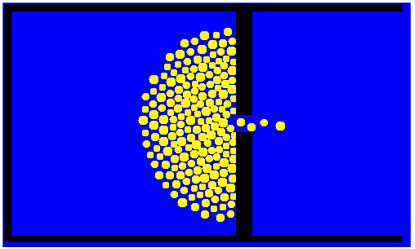
\includegraphics[width=60mm,keepaspectratio=true]{figures/column1.png}
		&
		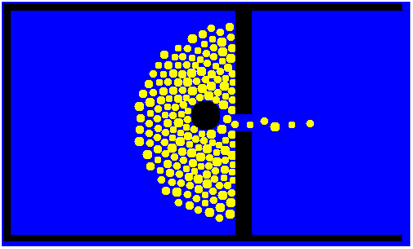
\includegraphics[width=60mm,keepaspectratio=true]{figures/column2.png}\\
		\hline
	\end{tabular}
	\caption{Unexpected emergence of scape patterns under different situations.}
	\label{tab:columnExit}
	\end{table}


ABM is most indicated for describing and simulating a system composed of “behavioral” entities. Whether one is attempting to describe a traffic jam, the stock market, voters, or how an organization works, ABM makes the model seem closer to reality. For example, it is more natural to describe how a party of hunters move in a terrain and circle their preys than to come up with the equations that govern the dynamics of the density of hunters. Because the density equations result from the behavior of hunters, the ABM approach will also enable the user to study aggregate properties.  

%TODO Pregunta al Xavi sobre això:
%	classical : social system → conceptualizations → person, people → abstractions (groups, social dynamics,...) → model the abstractions.
%	ABM : social system → conceptualizations → person, people → model the people.
%Classical : you need an extra step of inferited knowledge a priori

It is advisable, because it can be more natural and useful, to use ABM through the constituent units' activities under the next conditions.
\begin{enumerate}[i-] 
\item The behavior of individuals cannot be clearly defined through aggregate transition rates.
\item Individual behavior is complex. Everything can be done with equations, in principle, but the complexity of differential equations increases exponentially as the complexity of behavior increases. Describing complex individual behavior with equations becomes intractable. For instance, the individual copes with hysteresis, or there is heterogeneity in the set of behaviours or there are learning procedures and adaptability.
\item When the interactions between the agents are complex, nonlinear, discontinuous, or discrete (for example, when the behavior of an agent can be altered dramatically, even discontinuously, by other agents).
\item When space is crucial and the agents' positions are not fixed. Example: fire escape, trade, foraging in a stochastic spatial distribution of resources, traffic.
\item Activities are a more natural way of describing the system than processes.
\item Validation and calibration of the model through expert judgment is crucial. ABM is often the most appropriate way of describing what is actually happening in the real world, and the experts can easily “connect” to the model and have a feeling of “ownership”. 
\item Stochasticity applies to the agents' behavior. With ABM, sources of randomness are applied to the right places as opposed to a noise term added more or less arbitrarily to an aggregate equation. 
\end{enumerate}


Besides naturality in expressing models, ABM models are flexible. ABM can manage agents at different levels of aggregation. The decission units can be a person but also social entities like families, couples or tribes with their own rules for intearaction and behaviour. You can tune your model easily moving between different layers of abstraction from social sciences. ABM works with models where decission-making and aggregation is clearly separated. The range of complexity of the agent,  its behavior, degree of rationality, ability to learn and evolve, and rules of interactions can be tuned more independently of the range of complexity of the aggregation, individualality, and groups. This allows the modeller to work with different levels of description or complexity in the same model. %TODO ( explicar-ho mes???)

A last characteristic feature of agent computing, although not often noted, is that once a model has been created it provides not merely one aspect of the solution — the equilibria, say, or the stability — but rather entire solution trajectories \cite{Axtell2000}.\\
%%%%%%%%%%%%%%%%%%%%%%%%%%%%%

		    %aquests punts servirien per a justificar també perque triem ABMs i no un
		    %altre paradigma per a resoldre la nostra simulació
\subsection{ABM issues}

What is mentioned in a past section as a benefit must be mentioned here because there is an other side of the coin.
While other methods return only the equilibria or optimality conditions, ABMs yield trajectories of the
system, allowing to retrieve more data to induce patterns or any other dynamics that could emerge. This has its
drawbacks. For a causality result to be stablished or a pattern to be detected many runs must be performed.
If a result R appears as an outcome of the model, how strong are the bond of the result and that model? How
much does have to change the model to loose R? For equational models there are analytical methods to answer
the question. With ABMs many runs must be launched varying the initial conditions, testing parameter sensibility
and other protocols from model validation. This leads to computational expensive experimental tests. 
You have to come to terms with a post phase of analisys which could be computationally expensive, although improvements
in current computer technology begins to lower the concern.
\cite{Axtell2000}

Other computational costs that encumber the model are the decission processes, even more if we talk about AI and Problem Solving techniques with intensive cpu consumption.%TODO un pel curt




%%%%%%%%%%%%%%%%%%%%%%%%%%%%%%%%%%%%%%%%%%%%%%%%%%%%%%%%%%%%%%%

\chapter{Platforms / Software packages}
		\subsubsection{NetLogo...}

		    rasters -> +- automata
		    paralelism = 0
		    math libraries = 0?
		    ML, AI,... ???
		    -- efficiency
		    why do you not use netlogo

		\subsubsection{Pandora/Cassandra}

		Pandora : C++, STL, Python API
		Parallelism %transparent a l'usuari a traves de runtime generated code
	      
		The software we will use to implement the model is the Pandora Library, created by the social simulation
		research group of the Barcelona Supercomputing Centre. This tool is designed to implement agent-based 
		models and to execute them in high-performance computing environments (Rubio and Cela, 2010). It has been 
		explicitly programmed to allow the execution of large-scale agent-based simulations, and it is capable of 
		dealing with thousands of agents developing complex actions. The tool used has full GIS support to cope 
		with simulations in which spatial coordinates are relevant, as in the case here, where we want to detect 
		and compare spatial patterns. This library also allows the researcher to execute several simulations by 
		modifying initial parameters, as well as to distribute particular executions with high computer costs by 
		using a computer cluster. A cluster is formed by different linked computers (called nodes); the distribution 
		divides the computing cost of the execution between different nodes, each of which executes a part of the 
		entire simulation. As a result we will be able to run the simulation in a fraction of the time that would 
		be needed if we were using a single computer. The results of each simulation are stored in hierarchical data 
		format (HDF5), a popular format that can be loaded by most GIS. This feature is particularly useful, as we 
		will also use GIS to analyse simulation results.

		Finally, Pandora is complemented by Cassandra, a program developed to analyse the results generated by a simulation created
		with the library. 

		why do you use Pandora

\newpage 
\chapter{SugarScape vs Advanced Sugarscape} %% aqui veig mes clar que tota aquesta part funcionaria mes com un ODD


%% four our utility-based agents, justification : copied from Russel&Norvig_3rdEd, desplagia-ho
"Is it that simple? We just build agents that maximize expected utility, and we're done?" 
It's true that such agents would be intelligent, but it's not simple. A utility-based agent 
has to model and keep track of its environment, tasks that have involved a great deal of research 
on perception, representation, reasoning, and learning. The results of this research fill many 
of the chapters of this book. Choosing the utility-maximizing course of action is also a difficult 
task, requiring ingenious algorithms that fill several more chapters, Even with these algorithms, 
perfect rationality is usually unachievable in practice because of computational complexity, 
as we noted in Chapter 1.\\

%TODO fer matching dels features sugarscape amb les raons d'usar ABM que hi ha
%%			a la section sobre ABMs


%TODO  .. as proof case study
%SugarScape(Epstein) : environment for resource retrieval, social interactions, reproduction
%Match results, AI-agents are more proficient than their nonAI-counterparts


%		Perque comportaments + rics? l'approach classic es queda curt quan compliques les coses
%TODO		(add all the good features) (justifica-ho!, en que i com es queda mes curt?)
      
%		A question:
		  
%		  1.- do we get best results in our simulations adding deeper AI techniques to make richer
%		  the behaviour or decission making engines of the entities in the system? How should this be
%		  done?

%			\textbf{Sugarscape as test example for this hypothesis/topic}
		
%		  això ve del CS1... i ara us l'explico ( la pregunta 2)


%		  ( la 2 es mes per posar en contexte, la 1 es el topic, nomes existeix 1 pregunta)

%		We want to apply the trend begun with the announced motivation to the case study of Gujarat in
%Simulpast project. 	
		  Why HG survived more than expected? ( l'aplicacio de la pregunta 1)
			\textbf{interaction society vs envirm}
				2 main forces that drive change.
				Environment as a drive for adaptation.
				Society : safety network, cooperation and competition
\\
			\textbf{niche construction theory}
				AP occupy space and cause HG displacement.
\\
\\

%explica els agents com son a un ABM ( hauria de ser diferent d'un agent IA-Norvig que veiem mes endevant )
% busca models on puguis veure com son els seus agents, Journals, Hidden Order (llibre, el te la Cris)  


%ABM van be per a fer toy model, quan vols anar mes enlla i ser mes real, fa aigues --> cal IA.

%AI vs fake-AI : anar mes enlla de maquines d'estats, sistemes de regles, o mind mappings

%L'intere\'s d'aplicar AI es evitar hand-made minds. Hand-made mind pot portar un bias introduit pel dissenyador.
%Les opcions estan limitades als casos contemplats (disseny amb regles, xarxa semantica,.... posa mes exemples).
%Es busca una aproximacio mes SOFT i no tant hardwired com un sistema de regles (argumenta-ho MOLT,
%estaran els profes de la FIB, ¿Miquel Sanchez? has de rebatre molts paradigmes : Neurons, SVMs, CBRs, Production %Rules,...). 
%Menys bias, mes adaptatiu/flexible,... emergent i planificat.(llegeix llibres d'AI+SoftComp. ¿¿Copiar %justificacions de la SoftComputing + justificacions de ProblemSolving???)


Uncertainty \& Imprecision : state of resources(other foragers, climate stochacity),uncomplete know,... 
modelthinking{The complexity wrought by the increases in information, adaptability, and interconnectedness implies a lack of predictability about what's next}.

Logic Programming, Semantic Networks : hard to represent the foraging expertise of H.G. -> reduce the problem to 
resource adquisition -> math modelling -> maximization -> planning.

	  .- reactive, proactive...
	  .- adaptation
	  .- reasoning
	  .- planner

\subsection{Planners, ...}

	    UCT/MDP
	    policies
	    actions
	    sectors

	    approaches : greedy, plan next action, ?`adding lookahead?




	\section{What is SugarScape?}
	\section{Added advanced features}
		\paragraph{Same deduced trends and emerging dynamics}
		\paragraph{Realistic Adaptability to Parameter Perturbations}
	\section{Solving critics against classic SugarScape}
	\section{Experiments}

Made assumptions about behavior of real systems\\
  1st step, test if assumptions are reasonable\\
    -Validation, or representativeness of assumptions\\
  2nd step, test whether model implements assumptions\\
    -Verification, or correctness\\

La seguent comprovacio fes-la en el modelatge o un altre capitol mes adient:\\
Seed independence – random number generator starting value should not affect final conclusion (maybe individual output, but not overall conclusion)
Three key aspects to validate:
  -Assumptions
  -Input parameter values and distributions
  -Output values and conclusions





		\subsection{Initial Conditions}
			\subsubsection{Montecarlo?} 
			\paragraph{Emergence of stationary state; initial state := stationary state}
		\subsection{Experiment features}
			\paragraph{Description}
			\paragraph{Hypothesis}
			\paragraph{Assumptions}
			\paragraph{Config}
			\paragraph{Results}
			\paragraph{Validation}

\newpage 
\chapter{Gujarat Case Modelization} % ODD casi a pelo, comprovar les policies MDP,programmed,etc...
	\section{Introduction}
Northern Gujarat is a marginal environment between the Thar Desert and the more fertile area of Saurashtra. This region is an ecotone, characterized by the seasonal influence of the monsoon where contrasting ecological niches are in tension and small climatic shifts can generate significant environmental changes, eventually affecting  resource availability. Archaeological evidence points to the presence and possible coexistence in the area of groups of people with different resource management strategies and mobility behaviors: hunter-gatherers (HG); agropastoralists (AP); urban Harappans (UH).
The aim of this study is to model resource management and decision making among hunter-gatherer groups in this region to explore adaptive trajectories and performance in relation to a) environmental variability and b) the appearance of other specialized groups . 
What factors play a role in HG persistence or disappearance in arid margins? Is the advent of agro-pastoral behaviour a big enough change to explain the disappearance of HG behaviour? What happens when there is an external influence, such as that by UH? Does climate change affect HG behaviour?
	    \subsection{Hypotheses}
In our starting hypothesis HG groups are adapted to marked seasonality (due to monsoon) in the arid margins of northern Gujarat. We intend to explore HG resilience considering: a) the appearance of AP, b) the appearance of an external attractor (UH) and c) climate change. We define resilience as the ability of the system to maintain its identity in the face of internal change and external perturbation (Carpenter 2001).
	    \subsection{Aims and objectives}
	    \subsection{Knowledge Elicitation \& Brainstorming}
		\subsubsection{Interviews}
		\subsubsection{ECOTONO (journal club)}
		\subsubsection{ODD}

	\section{Physical World / Environment}		% put this section in Gujarat Case Study???
		\subsection{Statistical Modelling}
			\subsubsection{Data Sources}
			\subsubsection{Resource Pipeline}

	\section{Antrophological Model}				% put this section in Gujarat Case Study???
		\subsection{The Model}
			\subsubsection{Knowledge Represent}
				Arithmetics, logics, probab models,... which \& why

			\subsubsection{Decission Process}
				\paragraph{Hypothesis:richer agents}
				\paragraph{UPF hand to hand work:UCT algorithm}
				\paragraph{Methods}
				\paragraph{¿state of the art?}

			\subsubsection{Social Network}
				\paragraph{¿state of the art?}

			\subsubsection{Design}
				\paragraph{Organisational level design}
				\paragraph{Social structure}
				\paragraph{Interaction structure}
				\paragraph{Communicative structure}
				\paragraph{Normative structure}

			\subsubsection{Coordination level design}
				\paragraph{Action model}
				\paragraph{Task model}
				\paragraph{Agent model}
				\paragraph{Plan model}
	\section{Experiments}
		\subsection{Initial Conditions}
			\subsubsection{Montecarlo?} 
			\paragraph{Emergence of stationary state; initial state := stationary state}
		\subsection{Experiment features}
			\paragraph{Description}
			\paragraph{Hypothesis}
			\paragraph{Assumptions}
			\paragraph{Config}
			\paragraph{Results}
			\paragraph{Validation}


\newpage 
\chapter{Conclusion}
      \section{Achieved Objectives}
      \section{Achieved Objectives}
      \section{Comparison AI - Simple}
      \section{Difficulties \& Issues}
      \section{Publications/CAA}
      \section{Future Issues}
\newpage 

%TODO ordena la bibliografia per any
\chapter{Bibliography}
\begin{thebibliography}{13}

\bibitem{Epstein1999} 
	J.M. Epstein. 
	\emph{Agent-based computational models and generative social science. Generative Social
	Science: Studies in Agent-Based Computational Modelling}, pages 4-46
	1999

\bibitem{EpsteinAxtell}
	J.M. Epstein and R. Axtell.
	\emph{Growing Artificial Societies}, 1996.
	1996

\bibitem{Epstein2008}
	Joshua Epstein
	\emph{Why Model?}.
	2008.

\bibitem{Axelrod2003}
	R. Axelrod. 
	\emph{Advancing the Art of Simulation in the Social Sciences. Japanese Journal for Management Information System, Special Issue on Agent-Based Modelling}, Vol. 12, No. 3 
	Dec. 2003. 

\bibitem{Axelrod2007}
	R. Axelrod. 
	\emph{Simulation in Social Sciences. Handbook of research on nature-inspired computing for economics and management}, 1:90, 
	2007

\bibitem{JDoran}
	Doran, J., 
	\emph{Prospects for Agent-Based modelling in Archaeology}. Archeologia e Calcolatori, 10, 33-44.
	1999

\bibitem{RussellNorvig}
	Stuart Russell and Peter Norvig.
	\emph{Artificial Intelligence: A Modern Approach}
	2009

\bibitem{GilbertABM}
	Nigel Gilbert.
	\emph{Agent-Based Models}. SAGE Publications, California.
	2008

\bibitem{GilbertArtfSoc}
	Nigel Gilbert, Rosaria Conte.
	\emph{Artificial Societies. The computer simulation of social life}.
	1995.

\bibitem{TaberAndTimpone1996}
	Charles S. Taber, Richard J. Timpone.
	\emph{Computational modelling}.
	1996.

\bibitem{GilbertTroitzsch}
	Gilbert, N., Troitzsch, K.G.,
	\emph{Simulation for the Social Scientist}. Open University Press, USA.
	2008

\bibitem{Wooldridge2002}
	Michael Wooldridge.
	\emph{An Introduction to Multiagent Systems}
	2002

\bibitem{WooldridgeJennings1995}
	 Michael Wooldridge, Nick Jennings.
	\emph{Intelligent Agents: Theory and Practice}  Knowledge Engineering Review Volume 10 No 2. (c) Cambridge
	University Press 
	1995

\bibitem{Shoham1990}
	Yoav Shoham.
	\emph{Agent-Oriented Programming. Stanford University: Computer Science Department.(Technical Report STAN-CS-90-1335).}
	1990 

\bibitem{Lake}
	Lake, M W,
	\emph{2000. Computer Simulation of Mesolithic Foraging, in: Gumerman, G. J., Kohler, T.A. (Eds.), Dynamics in Human and Primate Societies: Agent-Based Modelling of Social and Spatial Processes}, Oxford University Press, New York, pp. 107-143.
\bibitem{Sugarscape}
	Sugarscape.
	\emph{http://ccl.northwestern.edu/netlogo/models/community/Sugarscape}

\bibitem{Pavon2008}
	Juan Pavón, Millán Arroyo, Samer Hassan, Candelaria Sansores.
	\emph{Agent-based modelling and simulation for the analysis of social patterns}. Pattern Recognition Letters 29(8): 1039-1048 
	2008

%\bibitem{Pidd2012}
%	Pidd
%	\emph{Pidd book}.
%	2012.
%\bibitem{Pidd2010}
%	Pidd
%	\emph{Pidd book}.
%	2010.
\bibitem{Pidd2003}
	Mike Pidd.
	\emph{Tools for Thinking: Modelling in Management Science, 2nd Ed. Wiley.Chichester,UK}.
	2003.

\bibitem{Robinson2008}
	Kathy Kotiadis, Stewart Robinson
	\emph{CONCEPTUAL MODELLING: KNOWLEDGE ACQUISITION AND MODEL ABSTRACTION}.
	2008.

\bibitem{Premo2010_pg31}
	L.S.Premo
	Equifinality and Explanation:The Role of Agent-Based Modeling in Postpositivist Archeology, published at Simulating Change; archeology into the twenty-first century Ed. Andre Costopoulos, Mark Lake. pg 31. First Column.
	2012.

\bibitem{Premo2010_EQF}
	L.S.Premo
	Equifinality and Explanation:The Role of Agent-Based Modeling in Postpositivist Archeology, published at Simulating Change; archeology into the twenty-first century Ed. Andre Costopoulos, Mark Lake. pg 31. Equifinality Leads to Underdetermination Among Alternatives.
	2012.

\bibitem{Premo2010_EXPLOR}
	L.S.Premo
	Equifinality and Explanation:The Role of Agent-Based Modeling in Postpositivist Archeology, published at Simulating Change; archeology into the twenty-first century Ed. Andre Costopoulos, Mark Lake. pg 33-34.
	2012.


\bibitem{PerezAndBatten2006}
	Pascal Perez and David Batten
	\emph{Complex Science for a Complex World; Exploring Human Ecosystems with Agents}. 
	August 2006.

\bibitem{GordonBurt2010}
	Gordon Burt
	\emph{Conflict, Complexity and Mathematical Social Science}
	2010.

\bibitem{Balci1988}
	Balci
	\emph{Balci book}.
	1988.
\bibitem{Heath2009}
	Heath
	\emph{Heath book}.
	2009.
\bibitem{Banks1998}
	Banks
	\emph{Banks book}.
	1998.
\bibitem{Davies2003}
	Davies
	\emph{Davies book}.
	2003.
\bibitem{Axelrod1997a}
	Axelrod
	\emph{Axelrod book}.
	1997.
\bibitem{TakahashiSallachRouchier2007}
	Takahashi, Shingo; Sallach, David; Rouchier, Juliette
	\emph{Advancing Social Simulation: The First World Congress, Springer, p. 354, ISBN 978-4-431-73150-4}.
	2007.
\bibitem{Bonabeau2002}
	Eric Bonabeau
	\emph{Agent-based modelling: Methods and techniques for simulating human systems, PNAS, vol 99} 
	2002.
\bibitem{Axtell2000}
	Robert L. Axtell
	\emph{WHY AGENTS? ON THE VARIED MOTIVATIONS FOR AGENT COMPUTING IN THE SOCIAL SCIENCES.The Brookings Institution}
	2000.
\bibitem{Helbing2000}
	D. Helbing, I. Farkas, and T. Vicsek 
	\emph{Simulating dynamical features of escape panic. Nature 407, pg 487-490.}
	2000.
\bibitem{MelanieMitchell2009}
	Melanie Mitchell
	\emph{Complexity, a Guided Tour.}
	2009.
\bibitem{Holland1997}
	John Holland
	\emph{Philosophica 59 (1997, 1) pp. 11-40. Emergence.}
	1997.
\bibitem{MillerPage2007}
	John H. Miller, Scott E. Page
	\emph{Complex Adaptive Systems: An Introduction to Computational Models of Social Life (Princeton Studies in Complexity)}
	2007.
\bibitem{Vicsek2002}
	Tamas Vicsek
	\emph{Complexity. The bigger picture. Nature 418, pg 131.}
	2002	

\bibitem{TakahashiSallachRouchier2007}
	Takahashi, S., Sallach, D., Rouchier J. (Eds.)
	\emph{Advancing Social Simulation: the First World Congress.}
	2007	

\bibitem{Gross2008}
	Claudius Gross
	\emph{Complex and Adaptive Dynamical Systems.}
	2008	
\bibitem{Dawkins1990}
	Richard Dawkins
	\emph{The Selfish Gene.Oxford University Press, 2nd edition}	
	1990

\end{thebibliography}

\end{document}
